\documentclass[a4paper]{report}

\usepackage[12pt]{extsizes} % Нестандартный размер кегля
\usepackage[russian]{babel} % Правильные переносы слов в конце строки
\usepackage[utf8]{inputenc} % Кодировка файла -- utf8
\usepackage{amsmath, amssymb} % Математические символы
\usepackage{bbold} % \mathbb{1}
\usepackage{fancyhdr} % Настройка верхних и нижних колонтитулов
\usepackage[usenames]{color} % Использовать названия цветов
\usepackage{lastpage} % Количество страниц в документе
\usepackage{enumitem} % Расширенные перечисления
\usepackage{titlesec} % Форматирование заголовков
\usepackage{titletoc} % Оглавление
\usepackage{csquotes} % Оформление цитат
\usepackage[document]{ragged2e} % Убирает отступ в абзатцах
\usepackage{graphicx} % Вставка картинок в файл
\graphicspath{{pics/}} % Узакываем путь до картинок
\usepackage{subcaption} % Подписи к картинкаи
\usepackage{multirow} % Объединение ячеек таблицы в одной колонке
\usepackage{wrapfig} % Обтекание таблиц и картинок текстом
\usepackage{xcolor} % Кастомные цвета
\usepackage{hyperref} % Ссылки
\usepackage{float} % Параметр H для фигур


\voffset=-20mm
\textheight=250mm
\hoffset=-20mm
\textwidth=180mm
\headsep=12pt
\footskip=40pt

\pagestyle{empty}
\cfoot{\large \thepage \ of \pageref*{LastPage}}
\renewcommand{\headrulewidth}{0pt}
\renewcommand{\footrulewidth}{0.4pt}
\fancypagestyle{fchapter}{
  \lhead{}
  \rhead{}
  \cfoot{\large \thepage \ of \pageref*{LastPage}}
  \renewcommand{\headrulewidth}{0pt}
  \renewcommand{\footrulewidth}{0.4pt}
}
\fancypagestyle{fstyle}{
  \headheight=30pt
  \footskip=30pt
  \lhead{\Huge \bf ML}
  \rhead{\large \leftmark}
  \renewcommand{\headrulewidth}{0.4pt}
  \renewcommand{\footrulewidth}{0.4pt}
}
\pagestyle{fstyle}

\renewcommand{\section}[1]{
  \refstepcounter{section}
  \vspace*{2em}
  \addcontentsline{toc}{section}{#1}
  {\bf\Large #1}
  \vspace*{1em}
}
\titleformat{\chapter}[hang]
  {\Huge}{Lecture \thechapter:}{1em}
  {\thispagestyle{fchapter}}
\renewcommand{\chaptermark}[1]{
  \markboth{Lecture~\thechapter: #1}{}
}

\addto\captionsrussian{
  \renewcommand{\contentsname}{Contents}
}
\titlecontents{chapter}[0em]{\vskip 0.5ex}{\bf\large}{\bf\large}{}

\definecolor{sapphireblue}{rgb}{0.06,0.32,0.73}
\hypersetup{
    colorlinks,
    linkcolor=sapphireblue,
    urlcolor=sapphireblue,
}


\begin{document}

\begingroup
  \hypersetup{linkcolor=black}
  \tableofcontents
\endgroup

\chapter{Introduction}

{\sf What is machine learning? The good answer is <<noone knows>>. However, we know whether or not this particular thing is machine learning or not. Another answer was proposed in the 90's by Arthur Samuel, one of the fathers of machine learning:
\begin{displayquote}
  \glqq It is a field of study that gives the ability to the computer to self-learn without being explicitly programmed.\grqq
  \begin{flushright}
  	A.L. Samuel
  \end{flushright}
\end{displayquote}
}

\section{Types of Machine Learning}

Here we can see some classification of mahine learning situations:
\begingroup
	\def\arraystretch{2}
	\begin{figure}[H]
		\centering
		\begin{tabular}{|c|c|c|} 
			\hline
			{\bf Type} & {\bf Small data} & {\bf Big data} \\
			\hline
			{\bf Panel data} & kNN, SVM, linear regression & boosted decision trees \\
 			\hline
 			{\bf Images, sound, text} & deep learning with tricks & deep learning \\
	 		\hline
	 		{\bf Cluster analysis} &  & clustering methods \\
	 		\hline
	 		{\bf Optimization} & Bayesian optimization & hill climb, annealing, GA\\
	 		\hline
	 		{\bf Agent systems} & q-learning & deep RL \\
 			\hline
		\end{tabular}
	\end{figure}
\endgroup
So the focus of this cource is practical knowledge. There is some theory to machine learning and in most situations theory doesn't work. <<Theory doesn't work>> means <<theory won't tell you what method is the best for particular task>>. Theoreticaly we can say that some method is better than other with probability 51\% but for particular task we may not know what method is the best. So you should know most of the algorithms and apply all of them for your task to find the optimal one.\\
Also there is an another classification of machine learning tasks -- classification by a data structure.

\subsubsection*{Supervised learning}

We have some dataset and we have superviser what tells us <<what is what>>, for example, we have some dataset of handwritten digits and superviser parses this digits. \\
So we have:
\begin{enumerate}[label=$\bullet$]
	\item $x$ -- input point
	\item $y$ -- output (or label)
	\item $f\colon X\to Y$ -- target function what we are trying to predict.
	\item $D=\{(x_1,y_1),\ldots(x_N,y_N)\}$ -- data for training; $x_i$ is the vector (for example, values of the pixel of the image), $y_i$ is the label of element $x_i$.
	\item $h\colon X\to Y$ -- hypothesis, the answer of our algorithm.
\end{enumerate}
Classification problem -- $y$ belongs to a set of classes.\\
Regression problem -- $y$ is a real valued number (or a vector).

\subsubsection*{Unsupervised learning}

Unsupervised learning is when you have only the datapoints $X$ and you want to extract some information, to get some insight into data structure, to get dependences or just for compressing. 

\subsubsection*{Semi-supervised learning}

Let's imagine you have some vector space and you have two data points: black and white. And you want to predict color for other points.

\subsubsection*{Active learning}

It is like semi-supervised learning, but we can ask for more labels but do it on a budget.

\subsubsection*{Reinforcement learning}

You don't have the dataset, you only have an environment and an agent that interacts with this environment and receives some revard. The task is find the best strategy for that environment.

\section{Instance-Based Learning}

In instance-based learning (also lazy learning) class $y$ of point $x$ will be
$$h(x, D)=\arg\max\limits_{y\in Y}\Gamma_y(x), \qquad \Gamma_y(x)=\sum\limits_{x_i\in D}\mathbb{1}(y=y_i)\cdot w(x_i,x)$$
where $D$ is our dataset, $w(x_i,x)$ weight of point $x_i$ for point $x$ (for example, distance between $x$ and $x_i$), $\Gamma_y(x)$ -- affinity of $x$ to class $y$.

\subsubsection*{Classifier evaluation}

Let's define for each class $y$ and our hypothesis $h(x, D)$:
\begin{enumerate}[label=$\bullet$]
	\item TP (true positive) -- number of points $x_i$ from dataset $D$ such as $h(x_i, D)=y_i=y$;
	\item TN (true negative) -- $h(x_i, D)\ne y$, $y_i\ne y$;
	\item FP (false positive) -- $h(x_i, D)=y$, $y_i\ne y$;
	\item FN (false negative) -- $h(x_i, D)\ne y$, $y_i=y$.
\end{enumerate}
Now we can define some metrics:
\begin{enumerate}[label=$\bullet$]
	\item Presicion (positive predicted value): $$\frac{TP}{TP + FP}$$
	\item Recall (true positive rate): $$\frac{TP}{TP+FN}$$
	\item False positive rate: $$\frac{FP}{TN+FP}$$
	\item Accuracy: $$\frac{TP+TN}{TP+FP+TN+FN}$$
	\item $F_1$ score: $$\frac{2}{\frac{1}{\text{Recall}}+\frac{1}{\text{Presicion}}}$$
\end{enumerate}

\subsubsection*{Train/Test}

If we have some hyperparameters of our classifier (for example, the number of neighbors in kNN), we want to find the optimal ones.
\begin{enumerate}
	\item Put aside a part of a dataset ($\approx 10\%-20\%$) for testing (test dataset);
	\item Train classifier on other part (training dataset);
	\item Optimize hyperparameters of classifier looking at the accuracy on the test dataset.
\end{enumerate}
If you have several different classifiers (and you want to find the best one for your task), it is a bad idea to compare them on a test dataset (what you used to find the best hyperparameters), because of overfitting. Put aside one more dataset (validation dataset).

\subsubsection*{Train/Validate/Test}

\begin{enumerate}
	\item Put aside a part of a dataset ($\approx 10\%-20\%$) for validation (validation dataset) and a part for testing (test dataset);
	\item Train classifier on other part (training dataset);
	\item Optimize hyperparameters of classifier looking at the accuracy on the validation dataset.
	\item Compare classifiers on the test dataset.
\end{enumerate}

\subsubsection*{Cross-validation}

If you have a small dataset, you want to use all your dataset for training and all your dataset for testing. And what we do is we shuffle the dataset, separate it into five parts and we make five experiments with same classifier hyperparameters (in k'th experiment we use k'th part for testing and others for training) and the acuracy will be the average of accuracies of each experiment.

\newpage
\subsubsection*{Pareto efficiency}

\begin{wrapfigure}{r}{0.25\linewidth}
	\vspace{-1.25cm}
  \begin{center}
    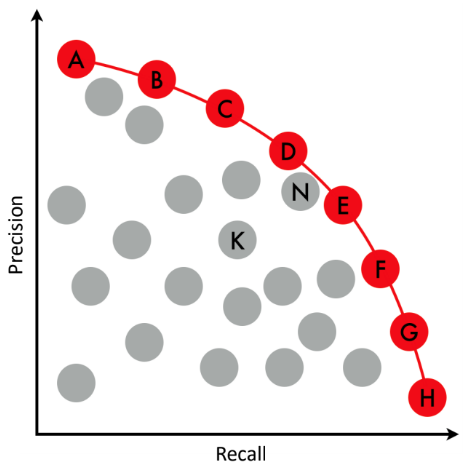
\includegraphics[width=\linewidth]{1a.png}
  \end{center}
  \vspace{-0.8cm}
  \caption*{(1.1) Pareto efficiency}
  \vspace{-1cm}
\end{wrapfigure}
Let's imagine we have some various classifiers and let's look on theirs presicion and recall [pic. 1.1.]. A classifier is Pareto efficient if there is no better classifier in terms of both presicion and recall (red points and point $N$). The red points are the first Pareto frontiers (point $N$ is one of the second Pareto frontiers, $K$ -- third).

\subsubsection*{Scalers}

If one feature goes from 0 to 1000 and the second feature goes from 0 to 1, then when we calculate distances between points, we will use only first feature. To fight that we can use scalers:
\begin{enumerate}[label=$\bullet$]
	\item MinMax scaler: $$x_{scaled}=\frac{x-\min(X)}{\max(X)-\min(X)}$$
	\item MaxAbs scaler: $$x_{scaled}=\frac{x}{\max(|X|)}$$
	\item Standart scaler: $$x_{scaled}=\frac{x-\text{mean}(X)}{\text{std}(X)}$$ where std$(X)$ is the standart deviation.
	\item Robust scaler: $$\frac{x-\text{median}(X)}{\text{percentile}_{0.75}(X)-\text{percentile}_{0.25}(X)}$$
	Robust scaler helps us to avoid points what are far from others.
\end{enumerate}
[Важное уточнение: если мы поделили датасет на две части (для обучения и для тестирования), то мы нормализуем не по всему набору данных, а отдельно для тестовой выборки и отдельно для обучающей.]

\subsubsection*{DROP5}

Prototype selection is calculating $h(x_i, D)$ not over all dataset $D$ but rather its subset $\Omega$. How we should select that subset? There are a lot methods and one of most popular is DROP5 (Decremental Reduction Optimization Procedure):
\begin{figure}[H]
  \centering
  \begin{subfigure}[c]{0.3\linewidth}
    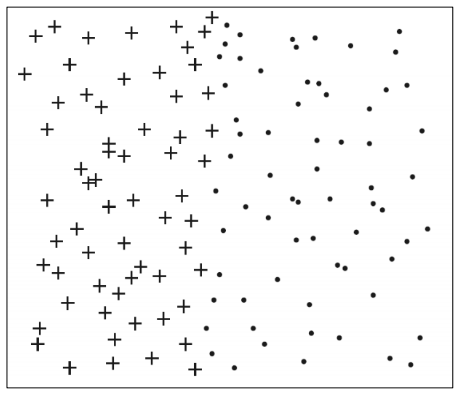
\includegraphics[width=\linewidth]{1b.png}
    \caption*{Dataset}
  \end{subfigure}
  \hspace{2cm}
  \begin{subfigure}[c]{0.3\linewidth}
    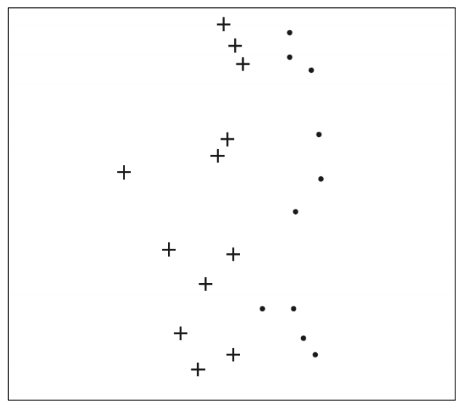
\includegraphics[width=\linewidth]{1c.png}
    \caption*{After DROP5}
  \end{subfigure}
\end{figure}
\begin{enumerate}
	\item Start with the full dataset.
	\item Sort data points, for example, by the number of neighbors from the other class.
	\item Go in the ascending order. Delete point $x$ if that does not increase the LOO error for the points that consider $x$ one of their closest neighbors.
\end{enumerate}

\section{kNN}

In kNN (k-nearest neighbors)
$$h_k(x, D)=\arg\max\limits_{y\in Y}\sum\limits_{x_i\in D}\mathbb{1}(y=y_i)\cdot w_k(x_i,x)$$
$$w_k(x_i,x)=\begin{cases}
	1, & \text{if $x_i$ -- one of the k nearest neighbors of $x$} \\
	0. & \text{otherwise}
\end{cases}
$$
Another variant is radius neighbors:
$$w_k(x_i,x)=\begin{cases}
	1, & \text{if distance $\rho(x_i,x)<R$} \\
	0. & \text{otherwise}
\end{cases}
$$
Actually we don't need a metric space, we only need $\rho(x_i, x)$ (distance between $x_i$ and $x$) to be defined. \\
And the way to evaluate how we are performing is to calculate leave-one-out-error:
$$LOO(k,D)=\frac{1}{|D|}\sum\limits_{x_i\in D}\mathbb{1}(h_k(x_i,D\backslash\{x_i\})\ne y_i)$$

\subsubsection*{WkNN}

Also we can use some other functions $w(x_i,x)=K(\rho(x_i,x)/r)$:
$$K=\max\Big(\frac{r-\rho(x_i,x)}{r}, 0\Big)\qquad K=q^{-\rho(x_i,x)}$$
where $r$ is some constant. We can define $r$ as a distance between $x$ and it's $(k+1)$ nearest neighbor.\\
Also there is a potential energy method:
$$h(x, D)=\arg\max\limits_{y\in Y}\sum\limits_{x_i\in D}\mathbb{1}(y=y_i)\cdot\gamma_i K\left(\frac{\rho(x_i,x)}{r_i}\right)$$
where $\gamma_i$ is some weight of point $x_i$, $r_i$ (influence range of point $x_i$) -- some constant. So we initialize $\gamma_i=0$ and after each step we change $\gamma_i$ ($\gamma_i\to\gamma_i+1$) if $h(x_i, D)\ne y_i$. And after some steps we stop.

\subsubsection*{Step-wise kNN}

If points of our dataset are from a big dimensional space, the euclidian distances between points may be huge. And if we also want to use kNN, the way to do it is the step-wise kNN:
\begin{enumerate}
	\item Select the best feature $k$ (what gives the best kNN result). Now we define the distance $\rho(x_i, x_j)$ between points $x_i$ and $x_j$ as the distance $\rho_k(x_i,x_j)$ between their k'th features.
	\item Find another best feature $k'$ and the weight $w_{k'}$ (what gives the best kNN result). Now we redefine $\rho(x_i,x_j)=\rho(x_i,x_j)+w_{k'}\rho_{k'}(x_i,x_j)$.
	\item Repeat second step while the LOO is decreasing (or the accuracy is increasing).
\end{enumerate}

\chapter{Clustering}

{\sf Usually we cluster points for information extraction, anomaly detection or data compression. How we use clustering for anomaly detection? We combine all the points, and those that are not included in the clusters are anomalies. How we compress data? Instead of having all points we can just have centroids of clusters. Also we can use clustering in active learning: we have an unlabeled data, we find a clustering, then ask for some labels and refine the clustering using that labels.}

\section{Clustering Algorithms}
\vspace{-0.6cm}
\subsubsection*{k-means}

The most widely used and the fastest algorithm is k-means. In this algorithm the number of clusters is predefined. And we want to minimize the variance:
$$\sum\limits_{x_j\in X}\min\limits_{\mu_i}\|x_j-\mu_i\|_2^2$$
where $X$ are points from our dataset, $\mu_i$ are centroids of clusters on current iteration. \\
So the algorithm is:
\begin{enumerate}
	\item Initialize $\mu_i$ randomly.
	\item Assign datapoint to cluster with the closest center.
	\item Shift $\mu_i$ to the center of mass of its claster: $$\mu_i=\frac{1}{|C_i|}\sum\limits_{x_j\in C_i}x_j$$
	\item Repeat second and third steps until convergence.
\end{enumerate} 
There are some problems with k-means. We may not know how many clusters we have. Also we can have a problem with initialization of cluster centroids: two points may lay into one cluster. To fight the last problem we can use k-means\texttt{++}.

\subsubsection*{k-means\texttt{++}}

\begin{enumerate}
	\item Select the first center randomly among the data points.
	\item For every $x$ calculate the distance $M(x)$ to the nearest center.
	\item Select the next center with probability proportional to $M^2(x)$.
	\item Repeat second and third steps $k-1$ times.
	\item Launch k-means.
\end{enumerate}

\subsubsection{Mean shift}

If the number of clusters is not predefined we can use mean shift algorithm.
\begin{enumerate}
	\item Initialize every point as its own cluster: $$\mu_i^0=x_i$$
	\item Then we shift every center of cluster to the center of mass of its neighborhood: $$\mu_i^{t+1}=\Big(\sum\limits_{x_j\in N(\mu_i^t)}RBF(x_j-\mu_i)\cdot x_j\Big)/\Big(\sum\limits_{x_j\in N(\mu_i^t)}RBF(x_j-\mu_i)\Big)$$ where $N(\mu_i)$ is some neighborhood of point $\mu_i$, $RBF$ is the Radial Basis Function: $$RBF(x-\mu)=e^{-c\|x-\mu\|_2^2}$$
	\item Repeat until convergence. Then merge close centers.
\end{enumerate}

\subsubsection*{DBSCAN}

This algorithm does not need a vector space (only distances to be defined). And the number of clusters is not predefined.\\
DBSCAN (Density-Based Spatial Clustering of Applications with Noice) is a simple algorithm. We define core samples -- data points that contain at least $m$ data points in their $\varepsilon$-neighborhood. Then we unite near (distance $<\varepsilon$) core samples in one cluster. Then we merge core samples and their neighborhoods.

\subsubsection*{Agglomerative clustering}

We initialize every point as its own cluster. And then at every step we merge two clusters. There are three strategies how to do that:
\begin{enumerate}
	\item Miminize variance of joined clusters.
	\item Minimize average distances between points in one cluster.
	\item Minimize maximum distance between points in one cluster.
\end{enumerate}
And we unite points until one cluster remains. After that we have some hierarchy of clusters: for every number of clusters we have such clusterization precalculated.\\
Also you can have a connectivity constraint like <<do not merge clusters if the distance between them is more than some constant>>.

\section{Clustering Metrics}

These metrics help us to answer the question <<How well we clusterize?>>:
\begin{enumerate}
	\item David-Bouldin index: $$DB=\frac{1}{n}\sum\limits_{i=1}^{n}\max\limits_{j\ne i}\left(\frac{\overline{\rho(\mu_i,x^i)}+\overline{\rho(\mu_j,x^j)}}{\rho(\mu_i,\mu_j)}\right)$$ where $\overline{\rho(\mu_k,x^k)}$ is the average distance between centroid $\mu_k$ and points in cluster $k$; $\rho(\mu_i,\mu_j)$ -- the distance between centroids $\mu_i$ and $\mu_j$.
	\item Dunn index. It is the minimum distance between two clusters divided by the maximum distance between points in one cluster: $$D=\frac{\min\limits_{i\ne j}\rho(\mu_i,\mu_j)}{\max\limits_{x_i,x_j\in\mu}\rho(x_i,x_j)}$$
	\item Purity: $$\frac{1}{|D|}\sum\limits_{C_i}\max\limits_{y}|x_j\in C_i,\ y_j=y|$$
	\item Classification metrics.
\end{enumerate}

\section{Comparison of Algorithms}

\begingroup
	\def\arraystretch{1.5}
	\begin{figure}[H]
		\centering
		\begin{tabular}{|c|c|c|c|c|}
			\hline
			K-Means & Mean Shift & \multicolumn{2}{|c|}{Agglomerative Clustering} & DBSCAN \\
			\cline{3-4}
			& & Variance & Average & \\
			\hline
			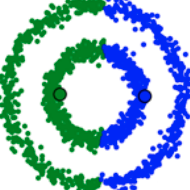
\includegraphics[width=0.15\linewidth]{2a.png} &
			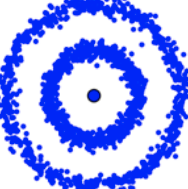
\includegraphics[width=0.15\linewidth]{2b.png} &
			
\includegraphics[width=0.15\linewidth]{2c.png} &
			
\includegraphics[width=0.15\linewidth]{2d.png} &
			
\includegraphics[width=0.15\linewidth]{2e.png} \\
			\hline
			
\includegraphics[width=0.15\linewidth]{2f.png} &
			
\includegraphics[width=0.15\linewidth]{2g.png} &
			
\includegraphics[width=0.15\linewidth]{2h.png} &
			
\includegraphics[width=0.15\linewidth]{2i.png} &
			
\includegraphics[width=0.15\linewidth]{2j.png} \\
			\hline
			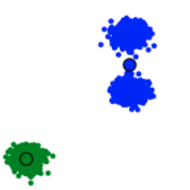
\includegraphics[width=0.15\linewidth]{2k.png} &
			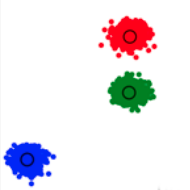
\includegraphics[width=0.15\linewidth]{2l.png} &
			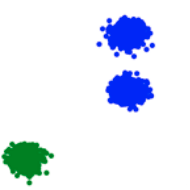
\includegraphics[width=0.15\linewidth]{2m.png} &
			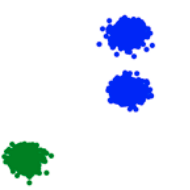
\includegraphics[width=0.15\linewidth]{2n.png} &
			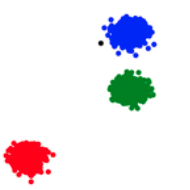
\includegraphics[width=0.15\linewidth]{2o.png} \\
			\hline
		\end{tabular}
	\end{figure}
\endgroup

\chapter{Desicion Trees}

{\sf Nothing to see here.}


<...>

\chapter{Ensemble Methods}

{\sf Ensemble method is just uniting the outputs of several classifiers into one. So let's say we have the three clasifiers (in that case you already familiar with KNN and Desicion Trees, you will be familiar with Support Vector Machines in a couple of lectures). We have three clasifiers and they have different outputs for different class in your space. You can merge those predictions into the one and have a unified answer. The simple way to do it is called voting.}

\section{Voting}

 The voting can be hard or soft; the first one when we just count the number of votes, for example, if I have five trees and most of them get class A as an answer, so my answer will be A class. If we have the even number of trees and the half of them say <<Сlass A is the answer>> and others say <<Class B is the answer>>, we have to deal with it by taking into account where they are not, you want the Higher Presicion or Higher Recall or just piking the classes in alphabetical order (the last one is the way it is done in Scikit-learn, so if you use this package, be aware of that). You can work around it by having an odd number of classifiers. Soft voting takes into account how sure the classifier in this desicion. For example, two classifiers get pair (0.1, 0.9) as an answer (0.1 is the probability of class A, 0.9 is the probability of class B) and three classifiers says <<Not sure>> (pair (0.51, 0.49)). The hard voting will give us class A as an answer (because last three get class A), however you see that that three trees don't actually give as an answer, because (0.51, 0.49) is so close to the neutral answer (0.5, 0.5). In soft voting you either end up the points for each class of the probablities, or you multiply, or you add, and then you can take an answer.

\section{Random Forest}

The one of the best algotithms which utilizes the voting system is called Random Forest, and just from the name of own you can guess that the classifiers are trees, but what makes it random? It is a sampling strategy. We only have our dataset, we don't have all the data points but let's simulate sampling from the general data by sampling from the dataset. And now let's build a tree for each sample and this will helps us find a noise. [Забегая вперед: мы строим каждое дерево не на всем объеме данных, а на какой-то его части. Эту часть мы будем выбирать исходя из некоторых весов точек. Сами веса при этом меняются после каждого построения дерева. Еще можно брать все точки, а веса как-то учитывать при построении деревьев.]\\
The greatest thing about random forest is the more trees you have the better random forest is: there is no owerfitting over the number of trees. So there are sampling strategies we mostly use the combination of bagging and random subspaces but let's just go through all of them.

\subsubsection*{Pasting}

Pasting is a simple sampling: let's take out of $N$ points $K$ random with no repeats.

\subsubsection*{Bagging (bootstrap agregating)}

The bagging (also bootstrap agregating) is a statistical term means the situation when you take the dataset of a sample with the same size but with repeats. Let's say we have the dataset with some features and two classes of the points from the dataset. Also we have weights for all points. That means that when we end up the error we multiply an error of every point by the weight of that point. The thing we gonna do the most today is manipulate that weight. \\
Let's imagine we want to take the points with repeats. If the sampling weights are the same, you can just take a random point. If the sampling weights are different and you want to sample with those weights, you can do the thing we did when we thought about how to sample in k-means$++$ algorithm. <...> \\
So you can use some weights in your classifier: when you build a tree, for example, you use the Gini formula ($\sum_{y\in Y}\frac{1}{|X|}\cdot|x: y(x) =y|\cdot|x: y(x) \ne y|$) but instead of counting the number of points you can add up their weights. There are different strategies for sampling; you can pick points according to the probability or you can just use this probability as your weights in your impurity calculation. Also instead of taking random samples of $N$ we can just assign a random numbers as weights and the best thing approximates bootstraping is a Poisson distribution so you can just select random numbers of the Poisson distribution and then use those numbers as weights in your impurity calculation.

\subsubsection*{Random subspaces}

The random subspaces is a way to try to randomize it and do a good work around noise anymore. We don't take random samples but rather we take random features so let's just use some subspace of features and random patches is both. So we use both random sample and random feature. Now you can natively calculate what is called feature importanse: if you want to now how important is your feature to the algorithm, you can build many trees and you can just calculate the number of trees that feature participates in. 

\subsubsection*{Extremely randomized trees}

Extremely randomized trees: instead of going over all the thresholds, over all the features, you can just say <<Ok, let's pick a hundred random thresholds and then pick the best>>. It doesn't work by itself, so if you want to construct one tree you will construct a really bad tree. However if you want to construct a forest, that not a bad idea. You can construct a good forest with extremly randomized trees.\\
{\it <Some talk about how random forests are good.>}\\
{\it <A meme slide about bootstraps and Munchausen...>}

\section{Boosting Algorithms}

Random forests constructs each tree basicaly independently, which is good because we can parellelize it. However, let's say we construct our first tree and it gives us a realy good answer with only a couple of problem points. In that case we would not want the next tree to be random, we would rather want the next tree to take into account the results of the first tree. The algorithms what do that are called Boosting Algorithms. It is important to know that we don't actually need to build a deep trees. So in the random forest we prefer to use trees with depth 5 or 6, and in adaptive boosting we use stumps (trees with only two leaves). In gradient boosting we use trees with depth 3 or 4. 

\subsubsection*{Adaptive Boosting}

So we have our dataset and the first thing we do is we construct the first classifier that gives us the answer. <...>\\
At the first step we do the weights is uniform, so every point has the weight $D_1(i)=\frac{1}{N}$. Then you build a tree to minimize error $E_t = \sum_{i=1}^N D_t(i) \cdot E(h_t(x_i), y_i)$ [в простом варианте $E(h_t(x),y) = 1$, если не угадали класс и $0$, если угадали]. So you just select the best threshold of all features and then you assign the weight $\alpha_t=\frac{1}{2}\ln(\frac{1-E_t}{E_t})$ for that tree. {\it <A little description of this function and how it helps us>} Now you need to recalculate weights:
$$\begin{cases}
D_{t+1}(i) = D_t(i)e^{\alpha_t}&\text{for incorrectly classified points,}\\
D_{t+1}(i)=D_t(i)e^{-\alpha_t}&\text{for correctly classified points.}
\end{cases}$$
Now you have the new sampling weights and you need to repeat the process, creating a new trees. You should stop if you don't have any improvement in your impurity, when you take into account the weights. The final hypothesys suggests the some number (hard voting) or the some number with coefficients (soft voting).\\
{\it <A slide with an example>}

\subsubsection*{Gradient Boosting}

When you want to get the best answer for your table data (not structured data like sounds, text, pictures etc) the best thing you can do is the gradient boostring.
\begin{displayquote}
  {\sf \glqq I think everyone sucks at explaining gradient boosting algorithms. Especially the authors of the gradient boosting algorithms.\grqq
  \begin{flushright}
    A.A. Shpilman
  \end{flushright}}
\end{displayquote}
It is one of most things that it is hard to understand and not hard but not easy to implement. It works, it has math behind it, but it's hard to understand why it works. There will be two explanations: one easy and one hard.
\begin{enumerate}
  \item[Easy:] This is the general formula for the gradient boosting:
  $$H_{t+1}(x)=H_t(x)+h_{t+1}(x)\to y \Rightarrow h_{t+1}(x)\to y - H_t(x)$$
  It is looks like the gradient descent. {\it <A little meeting with the gradient descent>} So we again build trees one by one, but we don't use stumps anymore. We use trees with the depth 3 (or 4, or 5, smth like that) and we will use regression, not the classification. So your tree predicts the numbers written in leaves [$H_t(x)$ -- число, записанное в листе, в котором <<лежит>> точка $x$, в дереве $t$]. How do we get the number in a leaf? We find average of all points that end up in this leaf [под суммированием точек подразумевается суммирование чисел, которыми мы обозначили классы точек, например для бинарной классификации это 1 и -1]. {\it <A slide with an example>} To get the next tree we need to subtract the number of each leaf of the previous tree from the points in this leaf and then we have the new y's [$h_{t+1}(x)$, новые классы точек]. <...> And then at some point you stop. That will give us the gradient booster: you take into account every new classifier, try to approximate the residual error and then you build the answer. The thing we noticed right away is that this way is bad and we need to have some learning rate [learning rate -- это коэффициент $\alpha$ в выражении $H_{t+1}=H_t(x)+\alpha h_{t+1}(x)$]. So we still fit the tree to the residual but we add it with some learnig rate $\alpha$ what is usually around 0.01--0.1. Why it works better? No one knows, this is a purely experimental result. {\it <Some intuition about this experimental result>} And the one more important thing is that usually gradient boosting starts with the first tree is just one leaf with the average, so you can just subtract the average right away. It is just centering the data. So again, gradient boosting, for just a regression, regression the error, it is the mean square error: $$MSE = \frac{1}{N}\sum(y-H_t(x))^2$$ <...> So we build the tree to minimize that error and for each leaf we define the weight is just the mean of all the values in that leaf. Simple. Works. Regression is very simple in terms of gradient boosting.\\
  {\it <Some talk about libraries. I'm not enough motivated to recognize that speech.>}
  \item[Hard:] What to do when it is not a simple regression, and we actually want to add some regularisation as well and that is where the complicated explanation comes in. So again:
  $$H_t=H_{t-1}(x)+h_t=\sum\limits_{j=1}^t h_j(x)$$
  In every step we want to calculate the $h_t(x)$. Also we want to minimize the error $E_t$:
  $$E_t=\sum\limits_{i=1}^{N}L(H_t(x_i),y_i) + \sum\limits_{j=1}^t \Omega(h_j)$$
  In our regression example the function $L$ is just a MSE. Also we have some regularization term $\sum_{j=1}^t \Omega(h_j)$. $\Omega(h_t)$ is usually just the number of leaves of a tree $t$.
  $$E_t=\ldots=\sum\limits_{i=1}^{N}L(H_{t-1}(x_i) + h(x_i),y_i) + \sum\limits_{j=1}^{t-1} \Omega(h_j)+\Omega(h_t)=$$
  $$=\sum\limits_{i=1}^N\left(2(H_{t-1}(x_i)-y_i)h_t(x_i)+(h_t(x_i))^2\right)+\Omega(h_t)+const$$
  In this formula we already know anything except $h_t$ and $\Omega(h_t$ what we are going to find in some steps in the gradient boosting process.\\
  In the general case $L$ is some differentiable function and you have:
  $$E_t=\sum\limits_{i=1}^N\left(L(H_{t-1}(x_i), y_i)+u_ih_t(x_i)+\frac{1}{2}v_i(h_t(x_i))^2\right)+\Omega(h_t)+const$$
  where
  $$u_i=\partial_{H_{t-1}(x_i)}\left(L(H_{t-1}(x_i), y_i)\right)$$
  $$v_i=\partial_{H_{t-1}(x_i)}^2\left(L(H_{t-1}(x_i), y_i)\right)$$
  In a case of regression: $u_i=2(H_{t-1}(x_i)-y_i)$, $v_i=2$. \\
  So as long as your error function is differentiable you can calculate a function what you are trying to approximate (like this: $L(H_{t-1}(x_i), y_i)+u_ih_t(x_i)+\frac{1}{2}v_i(h_t(x_i))^2$; you want to minimize $\sum_{i=1}^N \left(u_ih_t(x_i)+\frac{1}{2}v_i(h_t(x_i))^2\right) + \Omega(h_t)$).\\
  The regulirasation term $\Omega(f)$ in the case of extreme gradient boosting is the sum of all the leaves [слагаемое $\gamma M$, где $\gamma$ какая-то константа] plus sum of all the weights [$w_j$ -- число в листе $j$]:
  $$\Omega(f)=\gamma M+\frac{1}{2}\lambda\sum\limits_{j=1}^{M}w_j^2$$
  $$E_r=\sum\limits_{i=1}^{N}\left(u_iw_{q(x_i)}+\frac{1}{2}v_i(w_{q(x_i)})^2\right)+\gamma M + \frac{1}{2}\lambda\sum\limits_{j=1}^{M}w_j^2$$
  where $q(x_i)$ is the leaf of $x_i$.\\
  Then you can group that formula by leaves:
  $$E_t=\sum\limits_{j=1}^{M}\left(\sum\limits_{q(x_i)=j}u_iw_j+\frac{1}{2}\left(\sum\limits_{q(x_i)=j}v_i+\lambda\right)w_j^2\right)+\gamma M=\sum\limits_{j=1}^M\left(U_jw_j+\frac{1}{2}(V_j+\lambda)w_j^2\right)+\gamma M$$
  where $U_j=\sum\limits_{q(x_i)=j}u_i$ and $V_j=\sum\limits_{q(x_i)=j}v_i$ [$u_i$ и $v_i$ -- это те производные, что мы считали выше].\\
  So you have function $E_t$ to minimize and this is solution:
  $$w_j^{opt}=-\frac{U_j}{V_j+\lambda},\ E_t^{opt}=\gamma M-\frac{1}{2}\sum\limits_{j=1}^M\frac{U_j^2}{V_j+\lambda}$$
  This solution gives us the optimal weights to minimize our error when we constructing a tree. The Gain corresponding to that error is:
  $$Gain = \frac{1}{2}\left[\frac{U_{left}^2}{V_{left}+\lambda}+\frac{U_{right}^2}{V_{right}+\lambda}-\frac{(U_{left}+U_{right})^2}{V_{left}+V_{right}+\lambda}\right]-\gamma$$
  So it is how you pick the threshold. The gradient boosting still goes over all thresholds and picks the best. But now you just use this Gain formula. <...>
\end{enumerate}
The thing you need to understand is we didn't actually change anything between constructing the trees in the gradient boosting (but we can if we want to make some points more important than the others).\\
{\it <Smth about CatBoost>}\\
And the one important thing is that the learning rate ($\alpha$ in $H_{t+1}=H_t(x)+\alpha h_{t+1}(x)$) scales the answer of the tree.

\chapter{Linear Classifiers \& Theory of Error}

{\sf Let's say we have this dataset [pic. 5.1] with two features: a Plus class and a Minus class. If we use some sort of tree algorithm for this, we will get something like this [pic. 5.2]. <...> But ideally we want to separate the dataset with one line [pic. 5.3] (in case of $n$ dimentions it will be the $n-1$ dimentional hyperplane). <...>\\
\begin{figure}[h!]
  \centering
  \begin{subfigure}[l]{0.3\linewidth}
    \includegraphics[width=\linewidth]{5a.png}
    \caption*{(5.1) Dataset}
  \end{subfigure}
  \begin{subfigure}[r]{0.3\linewidth}
    \includegraphics[width=\linewidth]{5b.png}
    \caption*{(5.2) Tree algorithm separating}
  \end{subfigure}
  \begin{subfigure}[r]{0.3\linewidth}
    \includegraphics[width=\linewidth]{5c.png}
    \caption*{(5.3) Linear separating}
  \end{subfigure}
\end{figure}
}

\section{Linear Classifiers}

How do we separate? We define the hyperplane and the vector $w$ as the norm vector of that hyperplane and we multiply vector $x$ (from the dataset) by vector $w$. Then we find the threshold. If that\\ multiplication is over the threshold, we will say that $x$ in one class, and if it is under the threshold, $x$ will be in another class.
So this is a hypothesis [$h(x)$ возвращает $-1$ для класса Minus, $1$ для класса Plus]:
$$h(x)=sign\left(\langle w,x\rangle-threshold\right)$$
The one of the algorithms that utilise this hypothesis is called Perceptron.

\subsubsection*{Perceptron}

At the first step we should define a threshold and $w$. The vector $w$ is just a random vector. The threshold can be one of the coefficients of the vector $w$ (for example, $w_0$):
$$h(x)=sign\left(\langle w,x\rangle-w_0\right)$$
Then we can transform each vector $x$ of the dataset to simplify our $h(x)$ function: $$x=(x_1,\ldots,x_d)^T\to(1, x_1, \ldots, x_d)^T$$ After that transformation our hypothesis looks like that:
$$h(x)=sign\left(\langle w, x\rangle\right)=sign(w^Tx)$$
So we start with the random $w$ then we find such point $x$, when our hypothesis $h(x)$ does not match the answer $y$ (in case of two classes the hypothesis can be $1$ or $-1$). And then we just update $w$:
$$w_{new}=w_{old}+yx$$
[В конце концов после нескольких таких итераций мы остановимся. Гиперплоскость, перпендикулярная полученному вектору $w$ будет нашим ответом.]
Why would that work? Expalnation is quite simple: there is a theorem  that proves that it works in case of a linearly separable dataset. {\it <Some intuition about proof of this theorem>} And it actually works and works fast.

\subsubsection*{Pocket Algorithm}

If we have a linearly inseparable case, we have a Pocket Algorithm. {\it <An example with handwritten digits dataset>} A Pocket Algorithm is a simple modification of the Perceptron Algorithm: you just apply it for in given number of iterations and pick the best one in terms of validation dataset. It is called the Pocket Algorithm because you put your values in a pocket: when you find a new minimum you put it in the pocket and then you select the best partition from the pocket.


\hypertarget{new_features}{}
\subsubsection*{Feature Engineering}

The another way to fight a linearly inseparable dataset is adding new feature. For example [pic.~5.4] you can add feature like distance to (0,0) and get a linearly separable dataset [pic. 5.5].
\begin{figure}[h!]
  \centering
  \begin{subfigure}[l]{0.353\linewidth}
    \includegraphics[width=\linewidth]{5d.png}
    \caption*{(5.4) Dataset in $\mathbb{R}^2$}
  \end{subfigure}
  \hspace{2cm}
  \begin{subfigure}[r]{0.4\linewidth}
    \includegraphics[width=\linewidth]{5e.png}
    \caption*{(5.5) Dataset in $\mathbb{R}^3$}
  \end{subfigure}
\end{figure}

\section{Theory of Error}

However, the problem is how many new features can we add. The more features we have the more overfitting we have.

\hypertarget{ein_and_eout}{}
\subsubsection*{Error in sample and error out of sample}

Let's say we have a dataset with $N$ points ($x_1,\ldots,x_N$), a general set $X$ [которое является абстрактым множеством данных, которые мы хотим классифицировать, например, все люди на Земле и т.д.] and an error function $err$ that somehow defines. An error in sample is
$$E_{in}(h)=\frac{1}{N}\sum\limits_{i=1}^N err(h(x_i),f(x_i))$$
And an error out of sample is
$$E_{out}(h)=E_X[err\left(h(x), f(x)\right)]$$
where $f(x)$ and $h(x)$ returns a class of a point $x$ ($f$ is the target function, $h$ is our hypothesis), $E_{out}$ is the mathematical expectation of our error function on a general set $X$. [$E_{err}$ мы никогда не можем подсчитать напрямую, только оценить. На практике это делается через validation и test датасеты.]\\

\subsubsection*{Hoeffding's inequality}

There is the Hoeffding's inequality:
\hypertarget{gen_error}{}
$$P(|E_{in}(h)-E_{out}(h)|>\varepsilon)\le2e^{-\varepsilon^2N}$$
The difference $E_{in}(h)-E_{out}(h)$ is also called generalization error (sometimes in literature you can found $E_{out}$ as the generalization error). [The generalization error при заданном $h$ -- случайная величина в пространстве датасетов. Неравенство показывает, насколько хорошо ошибки гипотезы $h$ на датасетаx размера $N$ близки к ошибке $h$ на всем множестве $X$.] The big generalization error is a big overfitting and the small generalisation error is a small overfitting.\\
This inequality means for us that if we increase the dataset we exponentialy decrease the probability of overfitting for a one hypothesis. If we have a set of hypotheses then we have to multiply the right side by the $M$ -- number of hypotheses: 
$$P(|E_{in}(h)-E_{out}(h)|>\varepsilon)\le 2Me^{-\varepsilon^2N}$$
[В этом неравенстве $h$ -- лучшая из набора $M$ гипотез. Стоит отметить, что первое неравенство мы применять уже не можем: на разных датасетах лучшая из $M$ гипотез может быть разной.] If $M$ is small we can still guarantee mathematically that increasing the dataset does not get overfitting. Now the problem is how many hypotheses can we have. So this is a graph how our models behave ourselves in terms of complexity:
\begin{figure}[h!]
  \centering
  \begin{subfigure}[l]{0.7\linewidth}
    \includegraphics[width=\linewidth]{5f.png}
  \end{subfigure}
\end{figure}

\subsubsection*{From hypotheses to dichotomies}

Hovewer, even in a linear classification you don't have to go through all the hypotheses, for example, if you have some close hypotheses ($|E_{in}(h_1)-E_{out}(h_1)|\approx|E_{in}(h_2)-E_{out}(h_2)|$). So in terms of our math we'll go from hypotheses to dichotomies. The hypothesis is something that is defined for every point of the dataset and the dichotomy is also something that defined for every point of the dataset. But some dichotomies are not possible. [То есть некоторая гипотеза является дихотомией в зависимости от расположения точек из датасета относительно друг друга. К примеру, если вы используете для получения гипотез Perceptron Algorithm, то, чтобы некоторую гипотезу можно было назвать дихотомией, нужно чтобы в этой гипотезе классы были линейно отделимыми. В общем случае дихотомия типа H -- это гипотеза, которую можно получить алгоритмом H]. For example, if you set four points in four corners of the square, you will have only 14 dichotomies, because two dichotomies (where points in one edge have different class) you can not achive with Perceptron Algorithm. The actual number of the dichotomies is called the growth function:
$$m_H(N)=\max\limits_{x_1,\ldots,x_N}|H(x_1,\ldots,x_N)|$$
where $H(x_1,\ldots,x_N)$ is the set of possible dichotomies type $H$ on a points $x_1,\ldots,x_N$, $N$ is the number of points in the dataset. [Стоит понимать, что точки $x_i$ мы берем не из конкретного датасета. Мы берем все возможные расположения точек в пространстве (причем допускаются даже наложения точек друг на друга), считаем для каждого расположения количество возможных дихотомий, а затем берем макимум из подсчитанных значений.]

\subsubsection*{Vapnik-Chervonenkis inequality}

Now we can move from Hoeffding's inequality to Vapnik-Chervonenkis inequality:
$$P(|E_{in}(h)-E_{out}(h)|>\varepsilon)\le m_H(2N)\cdot4e^{-\varepsilon^{1/8}N}$$
The important thing that is now we have number of dichotomies that can be also exponential. And we still can't guarantee that in a big $N$ we will not overfit. However we can prove that the $m_H(2N)$ is almost always polynomial or less. How do we do that? 

\subsubsection*{Proof of polynomiality of a growth function in the presence of a breakpoint}

Well, the growth function is polynomial if it has what we called the breakpoint. The breakpoint is a $\min(k:m_H(k)<2^k)$ [Важно понимать, что для такого $k$ выполняется $\forall n\ge k\colon m_H(n)<2^n$]. In case of four points in 2D space, what we discussed already, $k=4$ is a breakpoint. <...> [Теперь перейдем к доказательству теоремы, используя новое понятие.\\
Пусть у нас есть набор из нескольких бинарных строк длины $N$, записанных в таблицу друг под другом ($i$-й столбец такой таблицы образован набором из $i$-тых символов всех строк). Известно, что для фиксированного $k$ выполнено следующее условие: если выбрать любые $k$ столбцов, то количество различных строк в выбранной части таблицы меньше $2^k$. Определим функцию $B(N,k)$ как наибольшее возможное количество строк в такой таблице.\\
Для начала покажем, что $\forall H\ B(N,k)\ge m_H(N)$, если breakpoint $m_H(N)$ равен $k$. Для этого убедимся, что все дихотомии типа $H$ длины $N$ можно вписать в таблицу с описанным правилом. Действительно, если у такой таблицы выбрать произвольные $k$ столбцов, то полученная таблица состоит из дихотомий длины $k$, значит, количество различных строк в выбранной части равно $m_H(N)<2^k$, что мы и хотели показать.\\
Теперь построим полиномиальную от $N$ оценку сверху на $B(N,k)$, тем самым получив ее и для $m_H(N)$. Для этого возьмем таблицу, удовлетворяющую описанным выше правилом, с наибольшим (т.е. равным $B(N,k)$) количеством строк. Разобьем строки этой таблицы на три части: $\alpha$, $\beta_+$ и $\beta_-$. Первая часть состоит из строк, у которых префикс длины $N-1$ уникален во всей таблице. Во вторую пойдут те из оставшихся, у которых последний символ равен $+1$, в третью, соответственно, $-1$. Таким образом $|\beta_+|=|\beta_-|=:b$. Обозначим $a:=|\alpha|$.\\
\begin{wraptable}{l}{5.8cm}
  \begin{tabular}{|c|c c c c|c|}
    \hline
    \multirow{5}{*}{$\alpha$} & +1 & +1 & $\ldots$ & +1 & +1 \\
                              & +1 & +1 & $\ldots$ & +1 & -1 \\
                              & $\vdots$ & $\vdots$ & $\vdots$ & $\vdots$ & $\vdots$ \\
                              & +1 & -1 & $\ldots$ & -1 & -1 \\
                              & -1 & +1 & $\ldots$ & -1 & +1 \\
    \hline
    \multirow{5}{*}{$\beta_+$}& +1 & -1 & $\ldots$ & +1 & +1 \\
                              & -1 & -1 & $\ldots$ & +1 & +1 \\
                              & $\vdots$ & $\vdots$ & $\vdots$ & $\vdots$& $\vdots$ \\
                              & +1 & -1 & $\ldots$ & +1 & +1 \\
                              & -1 & -1 & $\ldots$ & -1 & +1 \\
    \hline
    \multirow{5}{*}{$\beta_-$}& +1 & -1 & $\ldots$ & +1 & -1 \\
                              & -1 & -1 & $\ldots$ & +1 & -1 \\
                              & $\vdots$ & $\vdots$ & $\vdots$ & $\vdots$  & $\vdots$ \\
                              & +1 & -1 & $\ldots$ & +1 & -1 \\
                              & -1 & -1 & $\ldots$ & -1 & -1 \\
    \hline
  \end{tabular}
\end{wraptable}
Имеем следующее равенство:
$$B(N,k)=a+2b$$
Если мы возьмем префиксы длины $N-1$ строк из $\alpha\cup\beta_+$, то в полученной таблице любые $k$ столбцов образуют не более чем $2^k$ различных строк (поскольку таким свойством удовлетворяла исходная таблица). Значит:  
$$a+b\le B(N-1,k)$$
Теперь выберем префиксы длины $N-1$ строк из $\beta_-$. Заметим, что если в полученной таблице выбрать $k-1$ столбец, то различных строк в выбранной части будет меньше чем $2^{k-1}$ (иначе в исходной таблице столбцы с теми же номерами вместе с $N$-тым содержали бы не менее $2^{k-1}$ различных строк из $\beta_-$ и столько же соответствующих им строк из $\beta_+$, что в сумме дает $2^k$ различных строк, а это невозможно в исходной таблице по построению). Тем самым мы получили:
$$b\le B(N-1,k-1)$$
Суммируя последние два выражения, получаем:
$$B(N,k)=\alpha+2\beta\le B(N-1, k)+B(N-1,k-1)$$
Теперь мы можем показать следующую оценку:
$$B(N,k)\le\sum\limits_{i=0}^{k-1}\binom{N}{i}$$
Знаем, что $B(N,1)=1$, $B(1,k>1)=2$ и $\binom{N-1}{i-1}+\binom{N-1}{i}=\binom{N}{i}$, значит, использую индукцию по $N$ и $k$, можем показать:
$$B(N,k)\le B(N-1,k)+B(N-1,k-1)\le\sum\limits_{i=0}^{k-1}\binom{N-1}{i}+\sum\limits_{i=0}^{k-2}\binom{N-1}{i}=$$ $$=1+\sum\limits_{i=1}^{k-1}\binom{N-1}{i}+\sum\limits_{i=1}^{k-1}\binom{N-1}{i-1}=1+\sum\limits_{i=1}^{k-1}\binom{N}{i}=\sum\limits_{i=0}^{k-1}\binom{N}{i}$$
Последняя сумма является многочленом от $N$.]

\subsubsection*{VC-dimention}

$d_{VC}(H)$ for hypotheses type $H$ is the maximum number $N$ such that $m_H(N)=2^N$. If $k$ is the breakpoint, $d_{VC}=k-1$, so:
$$m_H(N)\le B(N,k)\le\sum\limits_{i=0}^{k-1}\binom{N}{i}=\sum\limits_{i=0}^{d_{VC}}\le N^{d_{VC}}+1$$
Why is this important? Because we can pull that in the Vapnik-Chervonenkis inequality and guarantee that we don't overfit in a big dataset. And the number $d_{VC}$ shows the effective complexity of a model.

\subsubsection*{VC-dimention for perceptron}

Now we prove that if $d$ is the space dimensionality, $d_{VC}=d+1$ [для случая, когда классы в дихотомии линейно разделимы].\\
So we have $d$ dimentions and at first we prove that we can have all the posible dichotomies for $d+1$ points. Let's construct the set of these points [не забываем добавить $d+1$'ую размерность, координата которой у всех точек из датасета равна 1]:
$$X=
\begin{pmatrix}
  x_1^T \\
  x_2^T \\
  x_3^T \\
  \ldots \\
  x_{d+1}^T
\end{pmatrix}
=
\begin{pmatrix}
  1 & 0 & 0 & 0 & \ldots & 0 \\
  1 & 1 & 0 & 0 & \ldots & 0 \\
  1 & 0 & 1 & 0 & \ldots & 0 \\
    &   &   & \vdots \\
  1 & 0 & 0 & 0 & \ldots & 1
\end{pmatrix}
$$
And we get invertable matrix, so we can solve this [обозначения как в описании Perceptron Algorithm: $y$ -- классы точек, $w$ -- нормаль к гиперплоскости, которую мы ищем]:
$$sign(Xw)=y;$$
$$Xw=y;$$
$$w=X^{-1}y.$$
Now we only need to prove that we can't have all hypotheses as dichotomies in $d+2$ points. So let's take $x_1,\ldots,x_{d+1},x_{d+2}$.  If two points from them are the same we already can't have all dichotomies. If there's not same points, let's assume that all hypotheses on that points are dichotomies. Because we work in $d+1$ dimentional space [$d+1$'ая размерность -- та, которая состоит из едениц] there is a vector $x_j$ that can be expressed to a linear combination of other $d+1$ vectors:
$$x_j=\sum\limits_{i\ne j}a_ix_i;$$
$$y_j=sign(w^Tx_j)=sign\left(\sum\limits_{i\ne j}a_iw^Tx_i\right).$$
If $y_i=sign(a_i)$ the $y_j$ can't be $-1$ (because $\forall i\ne j\ a_iw^Tx_i$ is always positive [так как $a_i$ и $w^Tx_i$ одного знака, поскольку мы так определили $y_i$]), so our assumption is incorrect and we prove the theorem.

\subsubsection*{Sufficient data}

So we proved that for perecptron algorithm:

$$P(|E_{in}(h)-E_{out}(h)|>\varepsilon)\le m_H(2N)\cdot4e^{-\varepsilon^{1/8}N}\approx N^{d_{VC}}e^{-N}$$

What does that give us? Well, if you want a nice hypothesis and if you don't want overfit you'd better have sufficient data: when $N\ge 10d_{VC}$ everything is OK. The problem is how to get the $d_{VC}$. For perceptron we have already get, for neural network we can calculate $d_{VC}$ as well because we can find the breakpoint. And what we do in the real world is the validation.

\section{Validation}

[Валидация -- процесс подбора оптимальных параметров обучающего алгоритма, используя заранее подготовленную для этого выборку. В отличие от валидации, тестирование и тестирующая выборка из датасета нужны для сравнения работы разных алгоритмов.]\\
Why is validation work? It works because dichotomy inequality works in it's original form, because we train our hypotheses on our dataset. So the validation is just pass the best hypothesis. There is an inequality for one hypothesis:
$$P(|E_{val}(h)-E_{out}(h)|>\varepsilon)\le2e^{-\varepsilon^2N}$$
Now the problem is: if you have many various parameters and so on then if you start pasting many hypotheses to your validation dataset you have to multiply right side by the number of hypotheses. That is why we go from validation to testing. That is why we train, validate and test. Because of Hoeffding's inequality. So you train on train dataset then you pass your answer on your validation dataset and you estimate the overfitting. The proper validation size is $K=\frac{N}{5}$ ($N$ is number of points in your dataset).

\subsubsection*{Cross-validation}

The problem with validation is we don't use all points. The validation dataset has only $20\%$ of all points and we don't use that points in our training. That is bad, because points are usualy expensive: you spend money for each point you have. So we do want to use them all. The thing what helps us is caled cross-validation.\\
The cross validation is the way to use all the points. We separate all dataset on 10 datasets, and take one of them as a validation dataset and all the others as a training dataset. And repeat. Now we should talk about data leaking.

\subsubsection*{Data leaking}

%Let's imagine you have a EEG signal from five pacients and you need to predict an epileptic seizure. The signals looks like this:\\
%{\it <One day there will be a pic>}\\
%And at some points in the EEG you have an epileptic seizures. You can say: Ok, let's have the validation dataset, let's have a trainig dataset. But you can divide your EEG diagrams like this:\\
%{\it <One day there will be a pic>}\\
%<...> What polutes your dataset. So you should divide like this:\\
%{\it <One day there will be a pic>}\\
{\it <Examples with EEG and MRT>}

\subsubsection*{Train $\rightarrow$ Validate $\rightarrow$ Test}

\begin{enumerate}[label=$\bullet$]
  \item Train the algorithm on your train dataset.
  \item Optimize hyperparameters on validation (or crossvalidation).
  \item Check the final perfomance on test.
\end{enumerate}

\chapter{Neural Networks}

{\sf An inspiration to a neural networks mashines comes from biological neural networks. In 1950's we already knew how it works. The the main thing that allows a neuron to filter all the useless signals that happend in the brain all the time is all-or-none law: if a signal exceeds the threshold potential, the neuron will give a complete response; otherwise, there is no response.}

\section{Perceptron}

So the perceptron works the same. However, it can be represented as the small neural network where input neurons are the signals what multiplied by some coefficients, then all results add up and if sum is over some threshold, we get the signal $+1$, otherwise, we get $-1$. The problem with that is we can only have one layer: if you combine several layers as how it happens in the brain, you will have no good way of training the multi-layer perceptron with the simple threshold function. So the way around it is replace the threshold function for something more complex. The first aproach is a single layer neural network with logistic function as a threshold.

\section{Single Layer Networks}

The single layer neural network with logistic function is called logistic regression. The logistic regression is the classification algorithm, not the regression algorithm. It's just called like that.

\subsubsection*{Logistic regression}

For the binary classification (with classes $+1$ and $-1$) the math comes out very nicely; the probability of the signal is the one minus the probability of the reverse signal:
$$P(y|x)=\begin{cases}
f(x)&\text{for }y=+1,\\
1-f(x)&\text{for }y=-1.
\end{cases}$$
This sigmoid function $\sigma$ satisfies the both parameters of $P(x|y)$:
$$P(y|x)=\sigma(yw^Tx),\qquad\sigma(s)=\frac{1}{1+e^{-s}},\qquad \sigma(s)=1-\sigma(s)$$
where $w^Tx$ is the answer of the perceptron in input $x$.\\
So if our output is the probability of classes, how would we calculate the loss function? How we would calculate the error what we can try to minimize? Well, we just use likelyhood:
$$\prod\limits_{i=1}^{N}P(y_i|x_i)=\prod\limits_{i=1}^{N}\sigma(y_iw^Tx_i)$$
Then we go from multiplication to sum of the logarithms and get loss function (what we will try to minimize) for the logistic regression:
$$L(w)=-\frac{1}{N}\ln\left(\prod\limits_{i=1}^N\sigma(y_iw^Tx_i)\right)=\frac{1}{N}\sum\limits_{i=1}^N\ln(1+e^{-y_iw^Tx_i})$$

Now the problem is training it. Even for one layer logistic regression we need to utilise the gradient descent:
$$w(t+1)=w(t)-\eta\frac{\partial C(w)}{\partial w}$$
The $C(w)$ is the cost function (instead it we can the use loss function; we typically talk about the loss function $L(w)$ (or $J(w)$) and the cost function $C(w)$). And we have the learning rate $\eta$.\\
In case of large data it becomes hard to calculate the average value of all logarithms in the loss function $L(w)$. However, we can go around by using a stochastic gradient descent: just calculate the loss function for batch (some part of the data) and then apply the gradient descent step for that batch. So if we use the stochastic gradient descent, at first we need to split our data into random batches and complete the gradient descent step for every batch. This iteration is called an epoch. The number of steps in one epoch is number of all points divided by the size of the betch ($N / N_{batch}$).
So this is the difference beteen the gradient descent and stochastic gradient descent:
$$\text{Gradient Descent: }w\leftarrow w-\eta\left(-\frac{1}{N}\sum\limits_{i=1}^N\frac{y_ix_i}{1+e^{y_iw^Tx_i}}\right)$$
$$\text{Stochastic Gradient Descent: }w\leftarrow w-\eta\left(-\frac{1}{N_{batch}}\sum\limits_{x_i\in batch}\frac{y_ix_i}{1+e^{y_iw^Tx_i}}\right)$$
Also we have a very stochastic gradient descent (when every bench contains only one point).\\
%$$w\leftarrow w-\eta\frac{\partial C(w^Tx_i,y_i)}{\partial w}$$
{\it <The reason why very stochastic gradient descent is not the best way>}

\section{Several Layers Networks}

So we have the algorithm for training in one layer neural network. The way to trainig the several layers is the back-propagation. 

\subsubsection*{Back-propagation}

At first we need to define some coefficients and numbers:
\begin{enumerate}[label=$\bullet$]
  \item $w_{jk}^l$ is the weight between neuron $j$ in layer $l-1$ and neuron $k$ in layer $l$.
  \item $x_j^l$ is the outcoming signal of neuron $j$ in layer $l$ after the activation function, i.e. $x_j^l=\sigma\left(\sum w_{ij}^lx_i^{l-1}\right)$ (for the logistic regression $\sigma$ is the sigmoid function). In the first layer $x_j^1=x_j$ ($x_j$ is a feature). You can look at all $x_i^l$ in other layers at the features as well (sometimes they called feature layers).
  \item $s_j^l$ is the incoming signal to neuron $j$ in layer $l$, $s_j^l=\sum w_{ij}^lx_i^{l-1}$
\end{enumerate}
So the values what we try to optimise is $w$'s. We want to calculate the gradient for loss functions over the $w$'s. This is the goldest way to calculate the partial derilivative of our loss function:
$$\nabla C_{w_{ij}^l}(w)=\frac{\partial C(w)}{\partial w_{ij}^l}=\frac{\partial C(w)}{\partial s_j^l}\times\frac{\partial s_j^l}{\partial w_{ij}^l}$$
Also we have
$$\frac{\partial s_j^l}{\partial w_{ij}^l}=x_i^{l-1}$$
because $s_j^l=\sum w_{ij}^lx_i^{l-1}$. Then we calculate $\delta_j^{l-1}$ what is defined as
$$\delta_j^{l-1}=\frac{\partial C(w)}{\partial s_j^{l-1}}$$
If the loss function $f$ is diferantionable then we just calculate all partial derilivatives for the last layer $L$:
$$\delta_i^L=\frac{\partial C(w)}{\partial s_i^L},\qquad C(w)=f(x^L),\qquad x_i^L:=\sigma(s_i^L)$$
[$x_i^L$ -- то, что возвращает нейрон $i$ из последнего слоя, вероятность принадлежности объекта классу $i$]. For the previous layers we can again apply the chain rule and calculate the $\delta_i^{l-1}$ using $\delta_i^l$:
$$\delta_i^{l-1}=\frac{\partial C(w)}{\partial s_i^{l-1}}=\sum\limits_{j}\frac{\partial C(w)}{\partial s_j^l}\times\frac{\partial s_j^l}{\partial x_i^{l-1}}\times\frac{\partial x_i^{l-1}}{\partial s_i^{l-1}}=\sum\limits_{j}\delta_j^l\times w_{ij}^l\times\sigma'(s_i^{l-1})$$
So back-propagation algorithm looks like this:
\begin{enumerate}[label=\arabic*.]
  \item Initialize weights randomly (with small random numbers in $[-0.1,0.1]$).
  \item Compute the forward path: calculate all $x$ and $s$.
  \item Go backward and calculate all $\delta$.
  \item Shift all weights: $w_{ij}^l\leftarrow w_{ij}^l-\eta x_i^{l-1}\delta_j^l$ ($\eta$ is some learning rate).
  \item Go to step 2.
\end{enumerate}
The important thing is you can calclulate all $\delta$ with tensors: you don't have to iterate over each coefficient but rather multiply tensors. Which is good because we can push it into the GPU's what are really good in multiplying thensors.

\subsubsection*{Activation functions}

Sigmoid: 
$$\sigma(s)=\frac{1}{1+e^{-s}}$$
Tanh:
$$\sigma(s)=\frac{e^s-e^{-s}}{e^s+e^{-s}}$$
Rectified Linear Unit (ReLU):
$$\sigma(s)=\max(0,s)$$
The sigmoid finction goes from 0 to 1. If you want something what can be negative you can use hyperbolic tangent what goes from $-1$ to 1. And if you want something what calculates very fast and doesn't get your gradient diminished when you reach big numbers you can use ReLU.

\subsubsection*{Softmax and cross-entropy}

In case of binary classification you use logistic function and you have one output neuron what gets the probability of one class. In multiclass classification case we utilize the function what is called the Softmax:
$$x_j^L:=\sigma(s_j^L)=\frac{e^{s_j^L}}{\sum e^{s_i^L}}$$
It is called Softmax because all last layer neurons output numbers around 0 (exept one that outputs number around 1).\\
The cross-entropy loss function is:
$$C(w)=-\sum o_i\log(x_i^L),\qquad o_i=\begin{cases}
1&\text{if }y=i,\\
0&\text{if }y\ne i.
\end{cases}$$
The fully conected network is the network when each neuron of the one layer connects with each neuron of the next layer and so on.

\section{Regularization}

Networks, espesualy fully conected, are very prompt to overfitting. For example let's say we have a very big network and train it to recognize images. Instead of learning features of the images, for example, recognizing a cat from a car by ears and so on, big neural networks can just memorize the images: it can looks on the value of concrete pixel. This is an overfitting -- memorising the dataset,  noise training and so on. How we can to regularize it? 

\subsubsection*{$L_2$ regularization}

When we regularize we trying to lower the VC-dimention, lower the number of possible hypotheses. We do that by adding some constraints to the loss function. Here we add the $L_2$ constraint:
$$C_{new}(w)=C(w)+\frac{\lambda}{2N}\|w\|_2^2$$
We want sum of the weight be the lowest possible. This way is called the $L_2$ regularization or weight decay.

\subsubsection*{Early stopping}

\begin{wrapfigure}{r}{0.4\linewidth}
  \vspace{-1.3cm}
  \begin{center}
    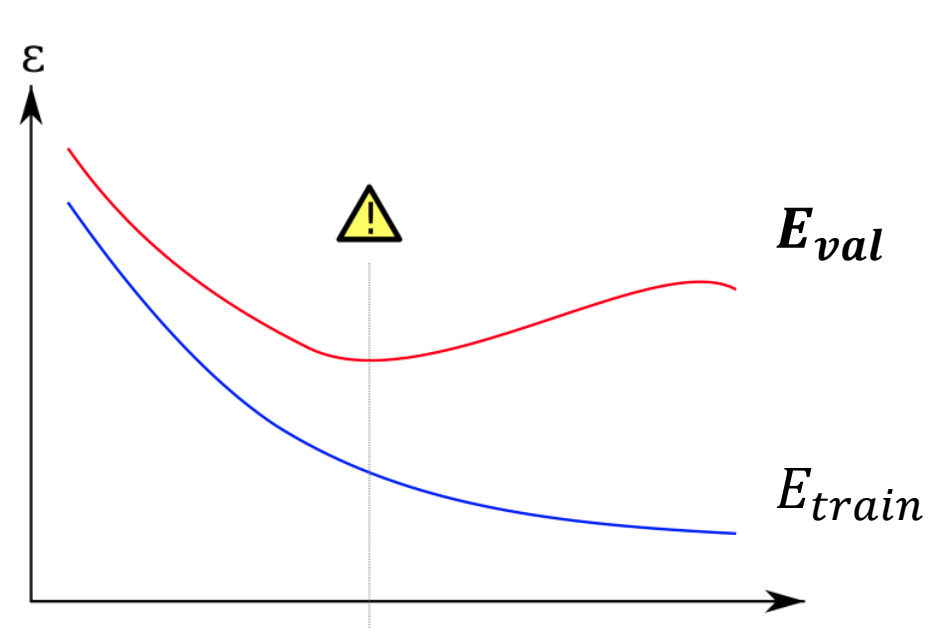
\includegraphics[width=\linewidth]{6a.png}
  \end{center}
  \vspace{-0.3cm}
  \caption*{(6.1) Early stopping}
  \vspace{-1.5cm}
\end{wrapfigure}
The another way in regularization is catching the moment of overfitting. So this is a typical graph [pic.~6.1] what shows gain between errors on the validation dataset and training dataset (the x axis is the number of epochs).\\
The error on the training dataset is always decrease, but error in the validation dataset in some point starts to increase. And at that point we want to stop (remember the weights of the network in that point).

\subsubsection*{Dropout}

Dropout is a direct way to preventing networks from memorizing the dataset. We just turn of some (50\%, for example) random neurons for every layers in every patch. The turned of neuron outputs 0. In that way the network will try to learn general features rather than specific pathways, because each pathway can be turned off.\\
\begin{figure}[h!]
  \centering
  \begin{subfigure}[l]{0.3\linewidth}
    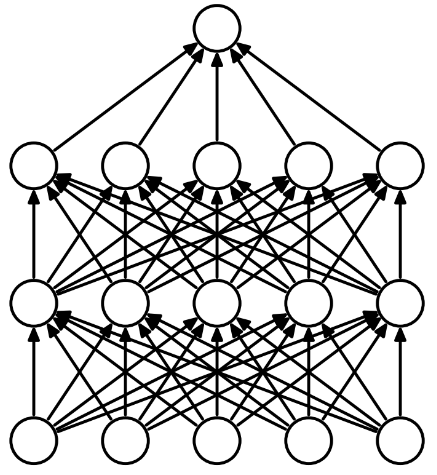
\includegraphics[width=\linewidth]{6b.png}
    \caption*{(6.2) Standart neural net}
  \end{subfigure}
  \hspace{2cm}
  \begin{subfigure}[r]{0.3\linewidth}
    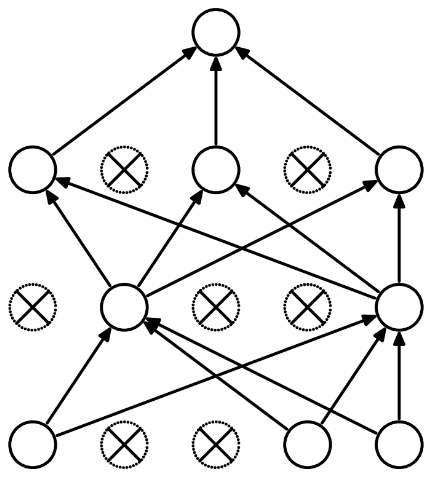
\includegraphics[width=\linewidth]{6c.png}
    \caption*{(6.3) After applying dropout}
  \end{subfigure}
\end{figure}
When we apply this network at some task we need to turn on all the neurons.

\subsubsection*{Data augmentation}

The overfitting doesn't happen if you have a lot of data. How to create a lot of data we will talk at the next lecture.

\section{Deep Learning Libraries}

If you don't like Python, learn to like Python because most of deep learning done in it. However there is still some inthusiasts what work on the deep learning for Java \href{http://deeplearning4j.org/}{library}.\\
Google represents \href{www.tensorflow.org}{TensorFlow} and the \href{keras.io}{Keras} (what is built on top of the first one). So if you just want to create networks simply you should use Keras. And if you want to create complex networks you should use TensorFlow.\\
The \href{torch.ch}{Torch} library easier than TensorFlow but more complex than Keras.

\chapter{Deep Learning for Images}

{\sf Let's imagine we have a fully connected network for image recognision and the problem is the bigger network we get the more connections the network has (more prompt of overfitting the network has, more computing pover needs for trainig). The main idea of deep learning is imposing a structure on that network. Rather than have a fully connected network we can have a structured network with less number of weights but more effective for solving specific task.}

\section{Convolution}

Deep leaning was enspired by biology. In the early 1950's professors David Hubel and Torsten Wiesel made \href{https://youtu.be/IOHayh06LJ4}{series of experiments} on cat's brain. They tried to answer how cats see the world around them, how their visual cortex works. The experiments were putting a cat in some locking mechanism, closing one eye of the cat that only annoys input from one eye. Then they drill a little hole in it's head and put an electrode at different place of the visual cortex to see how specific neurons reacts to specific visual stimulus. The cat saw some lines. So they found that some neuron best detects lines with one angle, while some others detects lines with another angle [\href{https://www.ncbi.nlm.nih.gov/pmc/articles/PMC1363130/pdf/jphysiol01298-0128.pdf}{ссылка} на статью для интересующихся].

\subsubsection*{Detecting lines}

So if a cat sees with lines let's ask neural network to see with lines. The detection of lines at various shapes was already known at that point and it was done in convolutions. The convolution is just pointwise multiplication and then addition it. You can see [pic. 7.1] the green tensor what is our input image, the yellow part of it is convolution filter and the red numbers are the values of this filter. What we do is we multiply each pixel value at red number and then we sum them up.\\
\begin{figure}[h]
  \centering
  \begin{tabular}{cccc}
    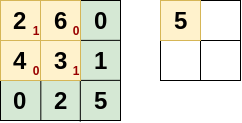
\includegraphics[width=0.2\linewidth]{7a.png} &
    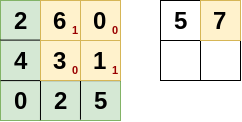
\includegraphics[width=0.2\linewidth]{7b.png} &
    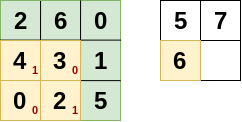
\includegraphics[width=0.2\linewidth]{7c.png} &
    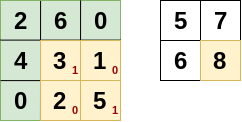
\includegraphics[width=0.2\linewidth]{7d.png} \\
    $2\cdot1+3\cdot1=5$ & $6\cdot1+1\cdot1=7$ & $4\cdot1+2\cdot1=6$ & $3\cdot1+5\cdot1=8$ \\
    & & & \\
    \multicolumn{4}{c}{(7.1) Convolution filter}
  \end{tabular}
\end{figure}
[В примере выше изображение было черно-белым: оно состояло из одного канала. Если же каналов больше, например, 3, то наш фильтр будет состоять уже из 3 слоев, необязательно одинаковых. Однако после прохода таким фильтром у изображения все равно останется один канал. Далее при указании размера фильтра я буду указывать размер одного слоя.]\\
So the parameters what we are trying to optimise are kernels (size of the filter) and strides (how large shift of the filter we use). You can see here [pic. 7.2] how various convolutions detect various feature of the image:\\
\begin{figure}[h]
  \centering
  \begin{tabular}{ccc}
    $ \begin{pmatrix}
      0 & 0 & 0 \\
      0 & 1 & 0 \\
      0 & 0 & 0 \\
    \end{pmatrix} $ &
    $ \begin{pmatrix}
      1 & 0 & -1 \\
      0 & 0 & 0 \\
      -1 & 0 & 1 \\
    \end{pmatrix} $ &
    $ \begin{pmatrix}
      -1 & -1 & -1 \\
      -1 & 8 & -1 \\
      -1 & -1 & -1 \\
    \end{pmatrix} $ \\
    & & \\
    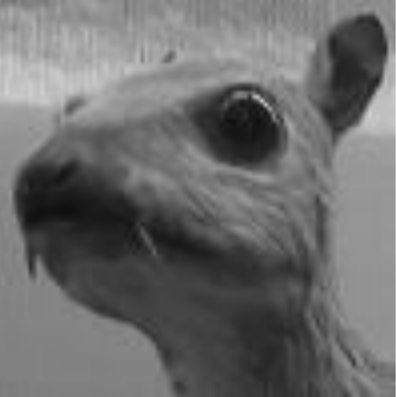
\includegraphics[width=0.2\linewidth]{7e.png} &
    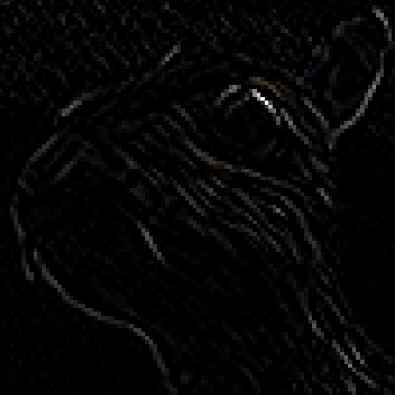
\includegraphics[width=0.2\linewidth]{7f.png} &
    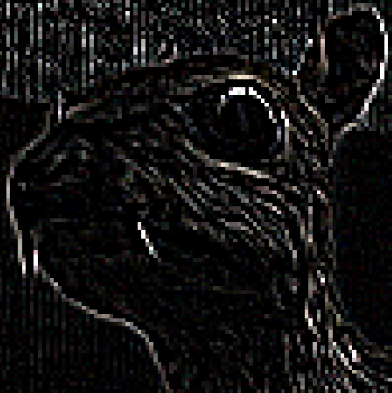
\includegraphics[width=0.2\linewidth]{7g.png} \\
    & & \\
    \multicolumn{3}{c}{(7.2) After applying some convolutions}
  \end{tabular}
\end{figure}

\subsubsection*{Convolution layers}

If you have simple shapes detecting then you can have the more complex shapes detecting. You can get that complex shapes detecting by applying convolution to the features you get after you apply convolution first time. And so on. So now we have a several convolution levels. What is important to understand that there is still neurons, there is still multiplication of preceptron input by weight. So all the math is still the same. When we back propagate the gradient we just sum not over all neurons but over specific neurons because all neurons in one convolution layer have the same weight.\\
Now let's imagine you have a typical image with size $224\times224\times3$ (3 because of color channels). It is called 2D convolution because it doesn't scan in depth. The next step is going over all image and take values what your filters outputs. And you have several different convolutions (every convolution has it's own filter). And what you get when you go with convolution over all picture is your convolved feature (or convolution map or your feature map). That black image with white edges of a deer is a convolution map. So you have set of some different maps and the next convolution layer looks at each map of the set like color channels (so it's still 2D convolution).\\
\begin{figure}[h]
  \centering
  \begin{subfigure}[l]{0.6\linewidth}
    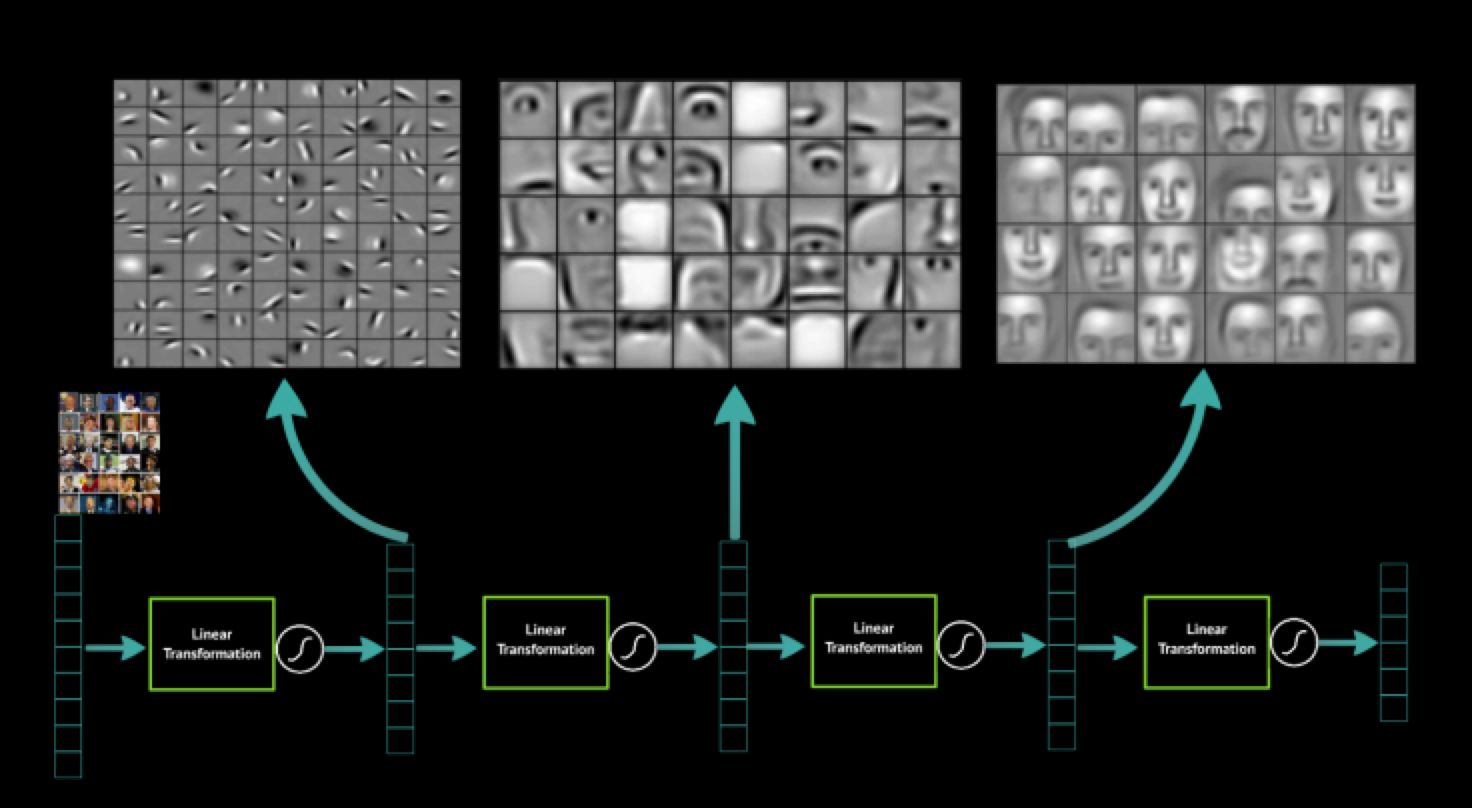
\includegraphics[width=\linewidth]{7h.png}
    \caption*{(7.3) Convolution layers}
  \end{subfigure}
\end{figure}

\vspace{-0.5cm}
\subsubsection*{Pooling}

The another operation what we use to decrease the complexity is called pooling. For example, if there is a clear signal on a some area of a feature map, then we just need a point with that signal because all the neightboring points probably are signaling the same. So we just take the maximum and it's called the maximum pooling. Also in some cases you can take average (and you'll have the average pooling).

\subsubsection*{Padding}

Padding is one way to perform convolution. For example, we have an image of size $M\times N$ and a filter of size $(2K+1)\times(2K+1)$. Before start moving the filter, we resize the original image to $(2K+M)\times(2K+N)$, adding a frame with weight $K$, consisting of zeros.

\section{Examples of Deep Neural Networks}
\vspace{-0.6cm}
\subsubsection*{LeNet-5}

The one of the first deep learning network. It was created in 1998 and it use all the algorithms and computer vision technics of that time. Also it used only 61470 weights. After that network there was a deep learning winter: almost noone works with them (except the several labs across the world) until 2012.

\subsubsection*{AlexNet}

In 2012 there was a ImageNet competition when AlexNet won by a huge margin with 15\% error (the result in 2011 were like 1st place had 27\%). This is the first deep network that proved to be so much ahead of everything else, and after that people start do all with deep learning.
AlexNet is a deep neural network what has 100,207,632 weights and it uses a GPU's calculations (what made this net successful in 2012). Also it has two parts each calculated individually on its own GPU. So there are some features of this net:\\
\begin{enumerate}[label=$\bullet$]
  \item Scales all images to $256\times256$, then takes random $224\times224$ batches and mirrors them.
  \item Substracts average pixel value from each pixel.
  \item ReLU ($\max(0,x)$).
  \item Dropout 0.5.
  \item Batch size 128, SGD with momentum 0.9 (momentum is how much of the previous gradient descent steps you keeps), L2 weight decay ($\lambda=0.0005$).
\end{enumerate}
The kernels on GPU 1 are largely color-agnostic, while the kernels on on GPU 2 are largely color-specific. This kind of specialization occurs during every run and is independent of any particular random weight initialization (modulo a renumbering of the GPUs) [\href{https://www.nvidia.cn/content/tesla/pdf/machine-learning/imagenet-classification-with-deep-convolutional-nn.pdf}{ссылка} на статью с более подобным описание для интересующихся].\\
Today we don't use the AlexNet, we use one of three things: VGGNet, Inception network or ResNet.

\subsubsection*{VGGNet}

VGGNet is a very deep convolutional network (VGG is the lab what invented it). The main idea is replace some layers of wide convolutions by more layers of $3\times3$ convolutions. It works because several layers of $3\times3$ have less weights than a big initial convolution. So it saves weights and it's very deep (but not heavy computantionaly). VGGNet is still used today in case of missing Google resources.

\subsubsection*{Inception network}

But is we have Google resources we can do something more complex. There are two main ideas of Inception network (it is named after the self-titled movie). The first is using $1\times1$, $3\times3$ and $5\times5$ convolutions in one layer and then concatenating the results. The second idea is to use $1\times1$ convolutions to made other filters flat. So there are inception modules:\\
\begin{figure}[h]
  \centering
  \begin{subfigure}[l]{0.4\linewidth}
    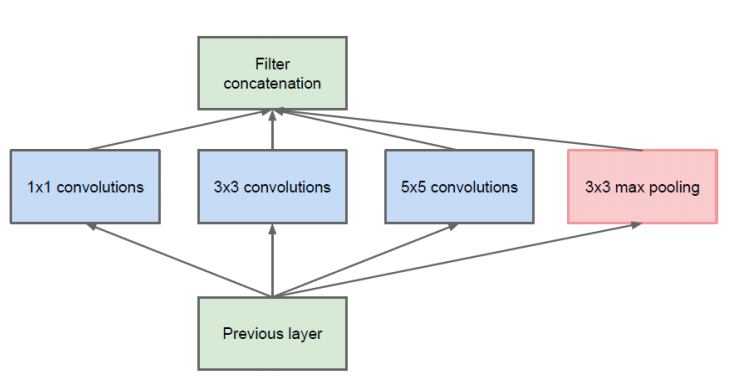
\includegraphics[width=\linewidth]{7i.png}
  \end{subfigure}
  \hspace{0.5cm}
  \begin{subfigure}[r]{0.4\linewidth}
    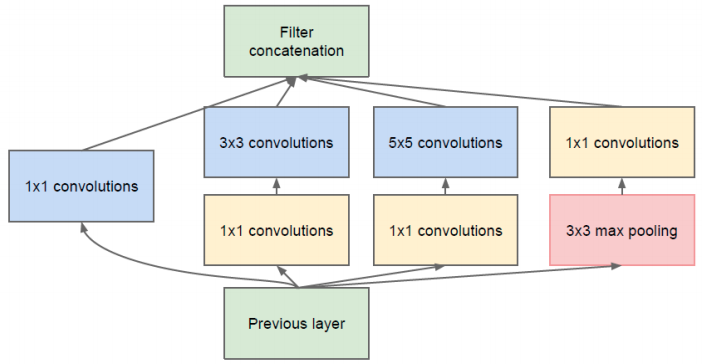
\includegraphics[width=\linewidth]{7j.png}
  \end{subfigure}
  \caption*{(7.4) Inception modules}
\end{figure}
And there are Inception network (also it named GoogLeNet):
\begin{figure}[h]
  \centering
  \begin{subfigure}[c]{0.7\linewidth}
    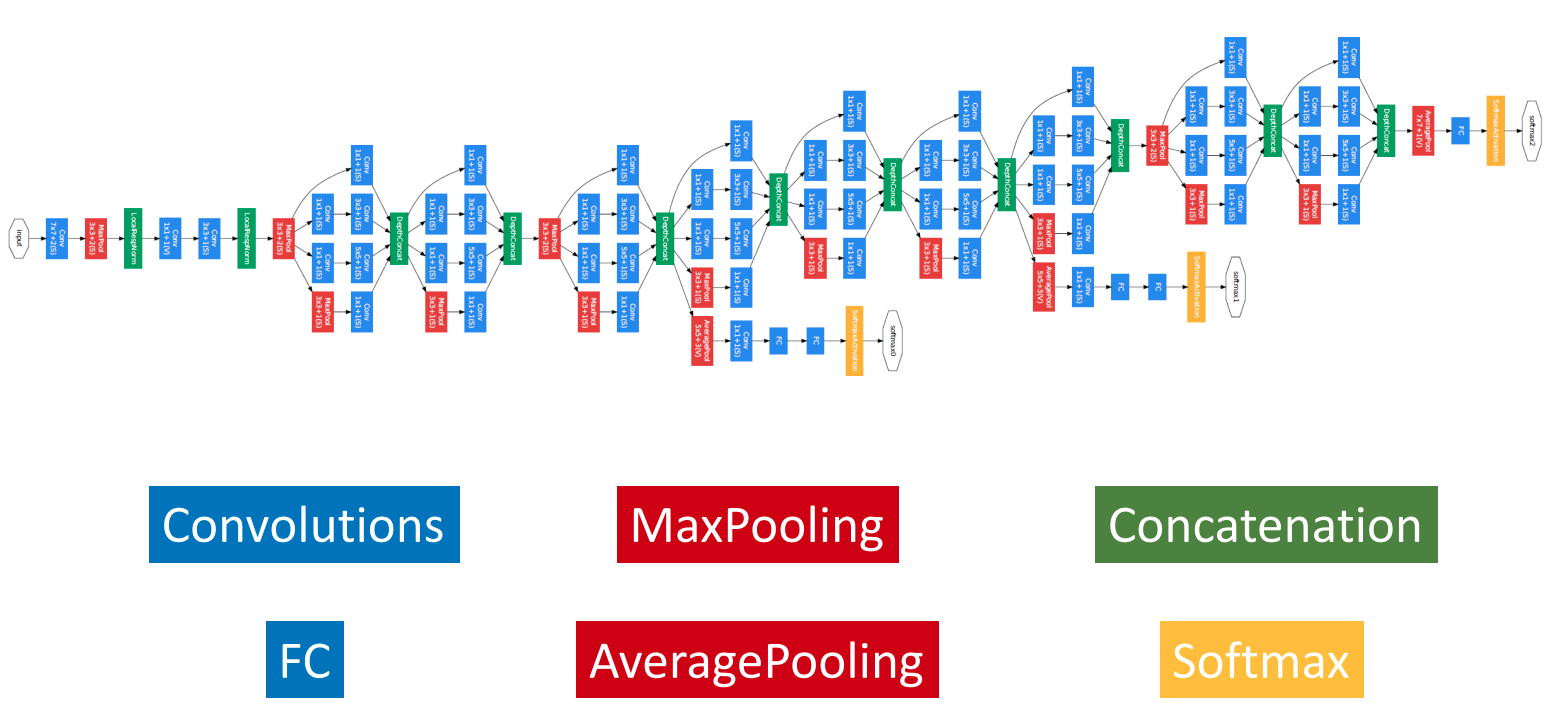
\includegraphics[width=\linewidth]{7k.png}
    \caption*{(7.5) GoogLeNet}
  \end{subfigure}
\end{figure}

\vspace{-0.5cm}
\subsubsection*{ResNet}

As you can see the GoogLeNet has multiple outputs. The reason is the information is lost the deeper you go --- it is nice to have an information from the different layers. But instead of it we can do additional information: add the output from the previous layer to the output of next layer. It is called a residual connection [pic. 7.6] (also called skip connections). Also we have a highway connection [pic. 7.7]: when you train in a separate neural network to determine how much of the output we add and how much of the previous input we keep.\\
\begin{figure}[h]
  \centering
  \begin{subfigure}[l]{0.31\linewidth}
    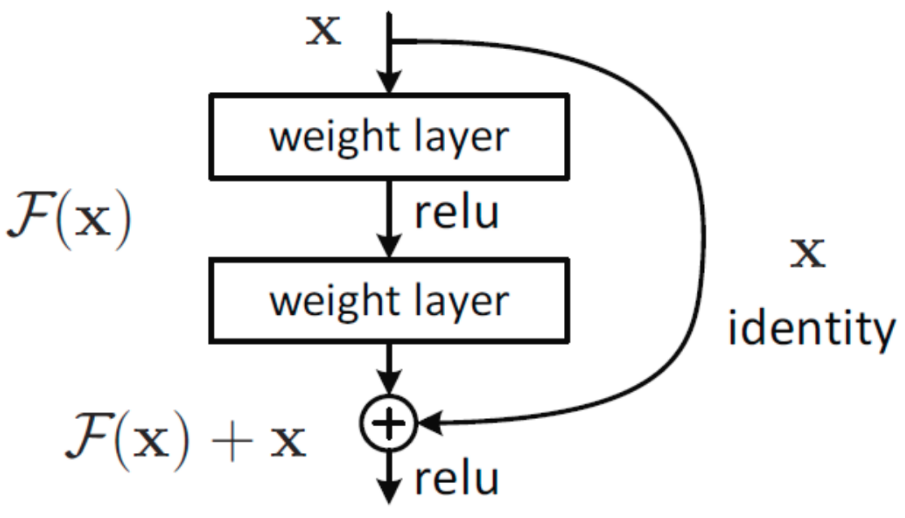
\includegraphics[width=\linewidth]{7l.png}
    \caption*{(7.6) Residual connection}
  \end{subfigure}
  \hspace{2cm}
  \begin{subfigure}[r]{0.4\linewidth}
    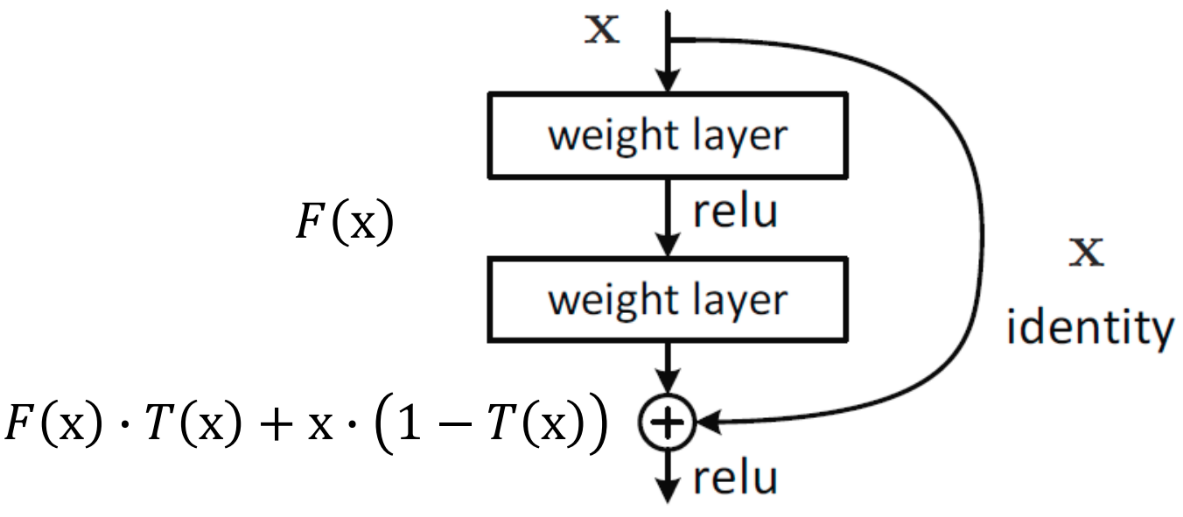
\includegraphics[width=\linewidth]{7m.png}
    \caption*{(7.7) Highway connection}
  \end{subfigure}
\end{figure}
So this ideas used in ResNet. ResNet is the widely used deep learning network. It has error rate only 3.57\%. However, if you want have less weights, you'll go to VGG: it still works well (now it has error rate 6.8\%).\\
The problem of that error rate is that human error rate is near 5\%. And error rate less than 5\% means the training on noice because all image dataset created by humans. So after the 2015 image networks changed from image classification to object detection.

\section{Technics in Image Analysis}
\vspace{-0.6cm}
\subsubsection*{Image augmentation}

The data is almost never enough. There is some ways to make your dataset bigger:\\
\begin{enumerate}[label=$\bullet$]
  \item Flip image. Be carefull, some flipped objects can be from another class: car upside down in come cases may be a trash.
  \item Rotate image. When you rotate, for example, on 45 degrees you may interpolate the result: fill the corners using a part of initial picture [pic. 7.8] or using the edge pixels of rotated image [pic. 7.9].\\
  \begin{figure}[h]
  \centering
  \begin{subfigure}[l]{0.2\linewidth}
    
\includegraphics[width=\linewidth]{7o.png}
    \caption*{(7.8) Symmetric}
  \end{subfigure}
  \hspace{2cm}
  \begin{subfigure}[r]{0.2\linewidth}
    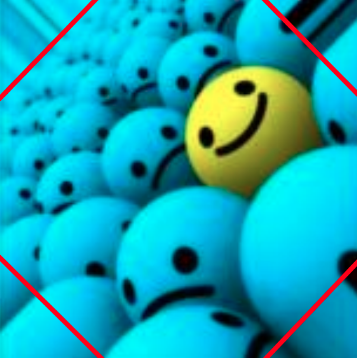
\includegraphics[width=\linewidth]{7n.png}
    \caption*{(7.9) Edge}
  \end{subfigure}
\end{figure}
  \item Crop image. This is very powerfull because it can get a lot of images.
  \item Scale image.
  \item Use Gaussian noice. After using a noice it becomes harder to overfit.
  \item Shift the colors by some constant. Good method of color shifting is transfering at the other color space and shiffting after that.
\end{enumerate}

\subsubsection*{Transfer Learning and Finetuning}

If image augmentation doesn't work, you have a transfer leaning. It is the most imprortant technic you can use on the image analysis. For example, someone has trained on ResNet and published all of it. The weights of his neural net is just a calculation of some image features. It doesn't matter what featers they are: dogs, cars etc; you can train on them. So the fransfer learning is training deep network on a big dataset, for example, ImageNet, then taking the result of that calculations as features, freeze it and training your small part for your specific task on output of the frozen part. It works wonderfully for any task, because there are so many features in the frozen part.\\
If you have many data you can use finetuning. The finetuning is like transfer learning but you don't fix other network weights. And you still train (finetune) to your task. Sometimes it helps but almost over it is overfitting becase the fisrt part is designed for millions and millions of images.

\chapter{Deep Learning for NLP}

{\sf Working with emages is quite simple in terms of image is already a vector or a tensor and you can just put it into your network. But words are more complicated. What is the word? Word is some sequence of letters with meaning. And close sequences can have opposite meanings. What we want to do is we still want to have a vector what we can feed into the neural network. And that is achived in word embeddings.}

\section{Word Embeddings}

Word embedding is creating vector representation for words from dictionary [обычно размерность пространства таких векторов берется в районе 100-300]. For example, we can create the vector space when some pathes have meaning: we take word <<queen>>, subtract the word <<woman>>, add the word <<man>> and end up with the vector of word <<king>>. Let's demonstrate how to achieve that.

\subsubsection*{word2vec (Google 2013)}

To create the vector from word we need some task that this vector should achieve. For example we can predict what words may surround a specific word $w_c$:
$$P(w_t|w_c)=\frac{e^{f(w_t,w_c)}}{\sum\limits_{w_i\in Dict}e^{f(w_i,w_c)}}$$
where $P(w_t|w_c)$ means the probability that some word $w_t$ is near the word $w_c$ ($f$ is some function). So after that we can calculate the loss function $J$:
$$J(w_c, T)=\frac{1}{|T|}\sum\limits_{w_t\in T}J_t,\qquad J_t=-\log P(w_t|w_c)=-f(w_t,w_c)+\log\Big(\sum\limits_{w_i\in Dict}e^{f(w_i,w_c)}\Big)$$
where $w_t$ are words in some neighborhood $T$ of word $w_c$. For example, in sentence <<Quick brown fox jumps over the lasy dog>> words <<quick>>, <<brown>>, <<jumps>> and <<over>> are neighbors for the word <<fox>>. So the word2vec method is let
$$f(w_t,w_c)=u_{w_t}^Tv_{w_c}$$
where $u$ and $v$ are word embeddings for words $w_t$ and $w_c$. Also every word $w$ has two vectors: one for calculations when $w$ is the target word (the first parameter of $f$) and one when $w$ is a center word (the second parameter of $f$). So we can initialize all vectors randomly and than shift them into correct ones by using gradient ascent. NOT descent, because we want to maximize the loss function! The terminology sometimes shifts...\\
But word2vec has a problem: every time we calculate the loss funcrion we need to sum up over all words in dictuary. Instead of that we can just select 5-10 samples of negative examples and sum up over them. This kind of word2vec is used in CBOW and skip-gram. In the first one we try to predict the word from the sum of the vectors of the surrounding words (to predict the center words from the contex). And the second one is trying to predict the context from the center word.

\subsubsection*{Fasttext}

A good increase in embeddings was fasttext from Facebook. They moved from embedding just for word to having the sum of embeddings for the word and all its possible n-gramms:
\begin{center}
	where $\to$ <where> + <wh + whe + her + ere + re>
\end{center}
where '<' and '>' are starting and ending symbols. This allows to have embeddings for that words what we did not encounter in our training process: embedding of a new word will be just a sum of embeddings of its n-gramms [да, без первого слагаемого, представляющего embedding всего слова целиком]. Also the number of n-gramms is much much less than number of words in a dictionary.

\subsubsection*{Sentence embedding}

It is still the same, you try to predict the next sentence from the vectors of words or you can just use sentence as the word.
The second way also works for protein sequences. They separated into 3-gramms in 3 ways: when you start from the first letter, the second and the third:
$$^{\color{red}(1)}M^{\color{blue}(2)}A^{\color{green}(3)}FSAEDVLKEYDRRRRMEAL..$$
$$\begin{cases}
	{\color{red} 1)} & MAF,SAE,DVL,KEY,DRR,RRM,..\\
	{\color{blue} 2)} & AFS,AED,VLK,EYD,RRR,RME,..\\
	{\color{green} 3)} & FSA,EDV,LKE,YDR,RRR,MEA,..\\
\end{cases}$$
So if you reduce dimensionality of received vectors, put 3-gramms on a map and paint them according to some chemical or phisical properties, you will see that it is able to extract the fisical or chemical information, for example, same mass, polarity etc:\\
\begin{figure}[h]
  \centering
  \begin{tabular}{ccc}
    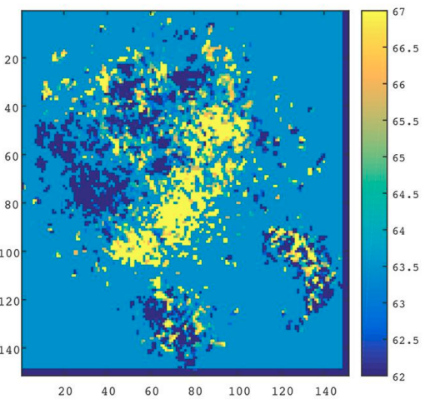
\includegraphics[width=0.25\linewidth]{8a.png} & \hspace{0.5cm}
    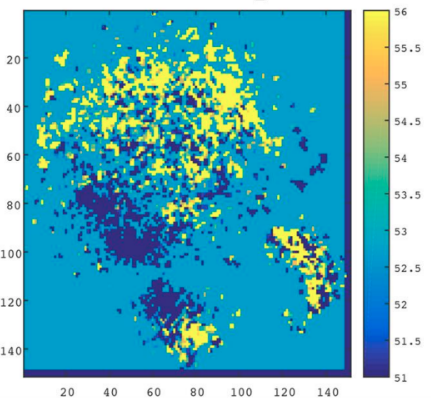
\includegraphics[width=0.25\linewidth]{8b.png} & \hspace{0.5cm}
    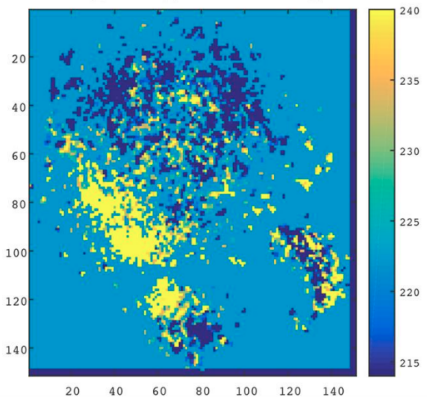
\includegraphics[width=0.25\linewidth]{8c.png} \\
    Mass & Polatiry & Hydrophobicy \\
  \end{tabular}
\end{figure}
That's amazing because you don't actually tell the computer that theese are protheins with letters correspondes to some chemical properties.

\section{Models in NLP}

The important thing is you don't have to use neural networks after you get embeddings. After you use deep learning technics to obtain your vectors you can use your vectors in trees or kNN etc. But if you want to do something complicated like mashine learning translation or text generation, you can use recurrent neural networks (RNN).

\subsubsection*{RNN}

The H's are networks, x's are inputs and y's are outputs [pic. 8.1]. Each network in RNN does not only produce an output but also some vector that it fits in the next same network. And for two years everyone got excited about recursive neural networks [pic. 8.2] but not anymore.\\
\begin{figure}[h]
  \centering
  \begin{subfigure}[c]{0.5\linewidth}
    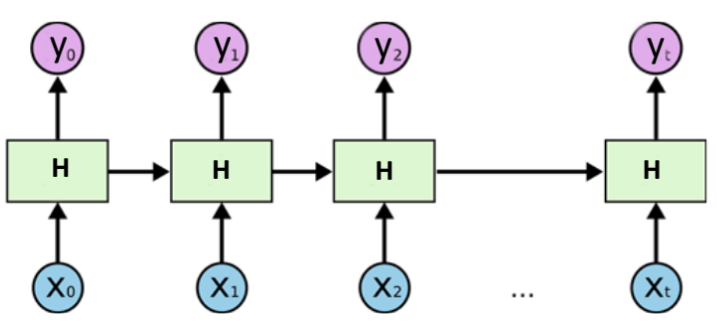
\includegraphics[width=\linewidth]{8d.png}
    \caption*{(8.1) Recurrent NN}
  \end{subfigure}
  \hspace{2cm}
  \begin{subfigure}[c]{0.3\linewidth}
    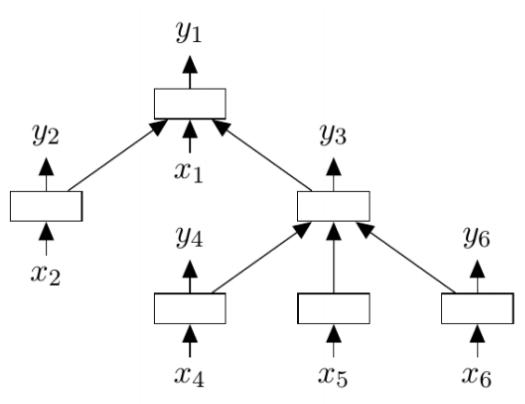
\includegraphics[width=\linewidth]{8e.png}
    \caption*{(8.2) Recursive NN}
  \end{subfigure}
\end{figure}
But the problems show themselves quite quickly after we start using RNNs and the almost always we have to do with vanishing or exploding gradient. {\it <The intuition why it happens>} To fight that the LSTM was envented.

\subsubsection*{LSTM, BiLSTM}

LSTM is a long short term memory network (we are going to go in depth over that network in a deep learning cource). What we need to know by now: it may helps when you have a sequentional data. The important thing is LSTM decides on each step what to keep from previous step, what to keep from current input and what to keep from current output.
\begin{wrapfigure}{r}{0.35\linewidth}
  \vspace{-1.4cm}
  \begin{center}
    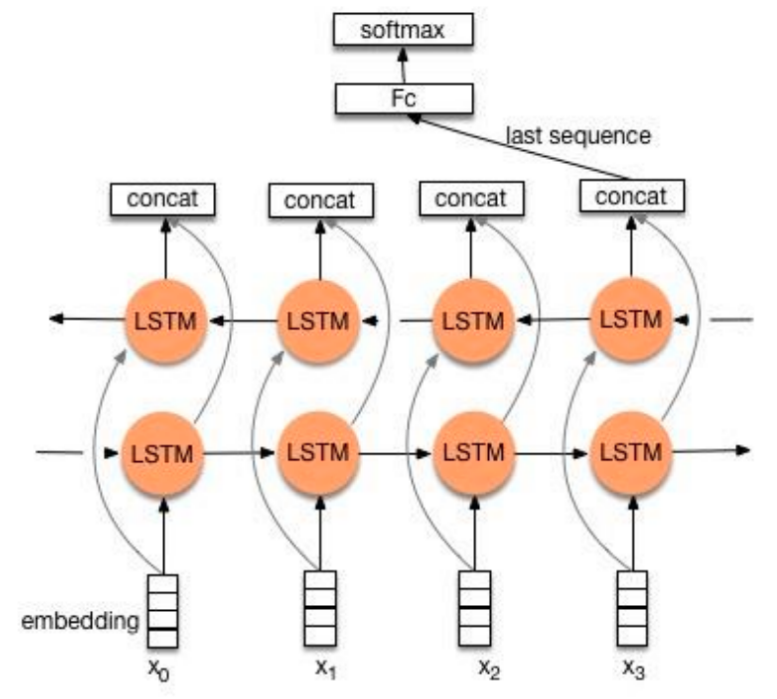
\includegraphics[width=\linewidth]{8f.png}
  \end{center}
  \vspace{-0.6cm}
  \caption*{(8.3) BiLSTM}
  \vspace{-0.8cm}
\end{wrapfigure}
How does LSTM looks in practice? It is a BiLSTM (bidirectional LSTM) [pic. 8.3]. Every word represented as a vector feeds into the first LSTM network and then you have another LSTM network what goes into other direction. So you read the text from front to back and from back to front and then feed outputs from the first network to the second. Then you concatenate both outputs and the result is a desicion for something. For example, if you want to generate the next word you can use softmax for the dictionary and then select the maximum. This is common used LSTM structure because you get more information when you go from left to right and from right to left.

\subsubsection*{Attention}

\begin{wrapfigure}{r}{0.35\linewidth}
  \vspace{-1cm}
  \begin{center}
    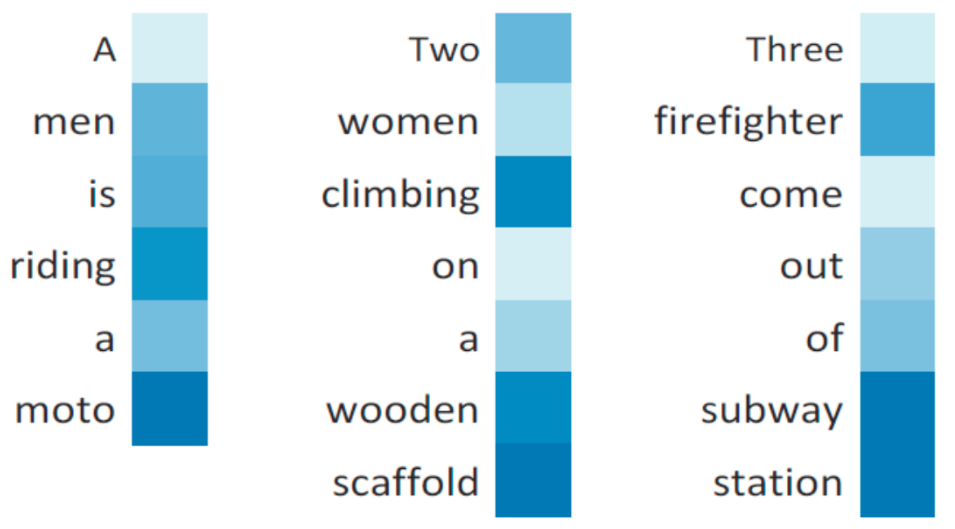
\includegraphics[width=\linewidth]{8g.png}
  \end{center}
  \vspace{-0.6cm}
  \caption*{(8.4) Attention}
  \vspace{-0.6cm}
\end{wrapfigure}
Attention is just adding a layer with the softmax after input layer. The property of the vector you get from softmax is that all the numbers of the features are summed up to one. It is called attention because you try to see how much attention every input gets. So you put your input into the attention layer, then you multiply the output of the attention network by the input and then you feed the result into desicion network. Here [pic. 8.4] you can see examples of distribution attention in a sentence. This picture does not show that men is more important than woman! The attention has meaning only in one sentence: <<climbing>> has more attention then <<two>> because it is more important for our decision. 

\subsubsection*{Transformers}

Transformers is a way to encode positional information and relationship. They have levels of input abstractions: query (Q), key (K) and value (V). For some tests your input is a query and key, sometimes it's value. We projected Q, V, K to various linear neural networks [идея в том, чтобы посмотреть на входные данные с разных сторон]. After that we use an attention to know how important is what we projected.\\
Another thing is a positional encoding. Positional encoding is adding some numbers to the input. Inputs with close positional encodings are close to each other and different positional encodings are far away from each other. You don't always have to use positional encodings. Sometimes it helps, sometimes it doesn't.

\section{Translation}
\vspace{-0.6cm}
\subsubsection*{Google neural machine translation}

How the mashine translation works now such as a Google mashine translation? Every time you write something to Google to be translated, your phrase goes into the eight GPUs (right now maybe more) and encoded into one vector that captures the meaning of the phrase. And that you decode that vector into another language one word by one. In this case you need examples of translations (parallel texts) for training.

\subsubsection*{Transation without parallel texts}

Facebook made very cool thing a couple mounthes ago. How to get translations if you don't have examples? How did they do that? They tried to push embeddings together. So you have one embedded space, you have another embeded space and let's made them look alike. Then we can switch a word embedding: one embedded language makes a vector from that word and another just decodes the result. How to push embeddings together?

\vspace{-0.3cm}
\subsubsection*{Adversarial learning}

Adversarial learning is when you work against another network. [Используется $N$ сетей, одна для каждого языка. Каждая сеть -- автоэнкодер, т.е. пытается на выходе получить ту же фразу, что и на входе. В середине этих сетей расположен слой небольшого размера, веса которого образуют embedding для фразы с input'а. Еще одна сеть, adversarial, смотрит на embedding вектора с этих слоев и пытается определить, к какой сетке (и, соответственно, к какому языку) они относятся. Ее награда (функция, которую мы максимизируем) -- то, насколько правильно она классифицирует. Награда каждой из $N$ сетей-автоэнкодеров -- сумма того, насколько она правильно восстанавливают фразу, и награды adversarial сети со знаком минус. Т.е. они помимо своей задачи восстановления последовательностей ище и стараются, чтобы вектора embedding были похожи. После обучения перевод из языка A в язык B выглядит следующим образом: мы берем первую половину сети-автоэнкодера для языка A и правую половину сети-автоэнкодера для языка B и конкатенацией получаем сеть, переводящую фразу.]

\vspace{-0.3cm}
\subsubsection*{Image Captioning}

The image captioning is just a translation from image to text. You have an images, you have a number of features and you decode that vector into text.

\chapter{Support Vector Machines}

{\sf Support vector machines (SVM) were a widely used method in 2000s. But it's still a very nice method when you have a small data problem. Let's imagine we have two classes ($+1$ and $-1$) and we have 3 possible hypotheses [pic. 9.1]. The red one is better than others. So SVM maximize the margins -- distances of the closest points of each class. It's mathematically proved that it's an optimal desicion. The bigger the margins then the higher the probability that we are correct on the general set. How do we solve it?}
\begin{figure}[h]
  \centering
  \begin{subfigure}[c]{0.4\linewidth}
    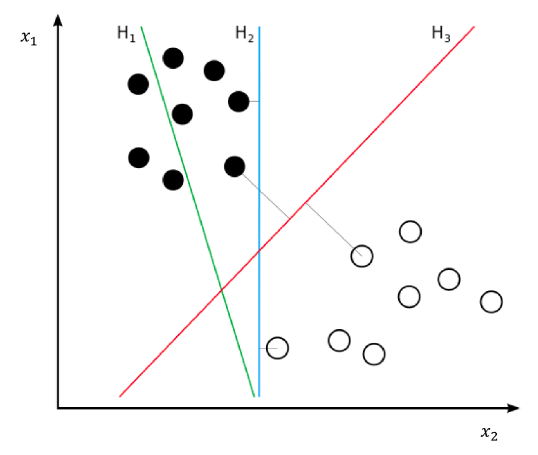
\includegraphics[width=\linewidth]{9a.png}
    \caption*{(9.1) Linear hypotheses}
  \end{subfigure}
  \hspace{2cm}
  \begin{subfigure}[c]{0.35\linewidth}
    \includegraphics[width=\linewidth]{9b.png}
    \caption*{(9.2) Maximize the margin}
  \end{subfigure}
  \vspace{-0.4cm}
\end{figure}

\section{Linearly Separable Case}
\vspace{-0.6cm}
\subsubsection*{Maximize the margin}

Let's say we have an optimal hyperplane $H$ what defined by a norm vector $w$ [pic. 9.2] (formula for $H$ is $w^Tx-b=0$). $H$ is optimal so the distances from $H$ to $x_j$ (closest point to $H$ from one class) and from $H$ to $x_i$ (closest point from another class) are maximal. The sum of that distances is the result of projecting $\overrightarrow{x_jx_i}$ on $w$ divided by $\|w\|$:
$$\frac{w^T(x_i-x_j)}{\|w\|}$$
what we want to maximize. Also $H$ is on the middle between $x_i$ and $x_j$ (because we want to maximize both distances $x_i$ to $H$ and $x_j$ to $H$). If we multiply $w$ and $b$ by same value, the $H$ will not change, so let's scale $w$ and $b$ such that hyperplane $wx-b=-1$ contains point $x_j$ ($w^Tx_j-b=-1$) and hyperplane $wx-b=1$ contains point $x_i$ ($w^Tx_i-b=1$). So we want to maximize:
$$\frac{w^T(x_i-x_j)}{\|w\|}=\frac{w^Tx_i-b-(w^Tx_j-b)}{\|w\|}=\frac{2}{\|w\|}$$
or, what is equal, minimize $\|w\|=w^Tw$ under $y_k(w^Tx_k-b)\ge 1$ constraints for every point $x_k$ from the dataset. That constraint means that point $x_k$ with $y_k=-1$ is in one subspace (when $w^Tx_k-b\le-1$) and with $y_k=1$ is in the other (when $w^Tx_k-b\ge1$). So this is an optimization task for SVM:
$$\begin{cases}
	\frac{1}{2}w^Tw\to\min, \\
	y_i(w^Tx_i-b)\ge1.
\end{cases}$$
The solution of this quadratic problem is quite easy, but we are going to do it in a complicated way.

\subsubsection*{Karush-Kuhn-Tucker conditions}

So we have an optimisation task (what is called the primal problem):
$$\begin{cases}
	\min\limits_{z}f(z), \\
	g_i(z)\le0, \\
	h_i(z)=0.
\end{cases}$$
If $z^*$ is a local minimum, then there are Lagrangian multipliers $\alpha_i^*$ and $\beta_j^*$ for:
$$\mathcal{L}(z,\alpha,\beta)=f(z)+\sum\limits_{i=1}^{m}\alpha_i g_i(z)+\sum\limits_{j=1}^{n}\beta_jh_j(z)$$
such that (Karush-Kuhn-Tucker conditions):
$$\begin{cases}
	\frac{\partial}{\partial z_i}\mathcal{L}(z^*,\alpha^*,\beta^*)=0, \\
	\frac{\partial}{\partial \beta_i}\mathcal{L}(z^*,\alpha^*,\beta^*)=0, \\
	\alpha_i g_i(z^*)=0, \\
	\alpha_i^*\ge0.
\end{cases}$$
And finding the solution of the primal problem is equal to finding the solution of the dual problem (if both solutions exists):
$$\max\limits_{\alpha,\beta}\min\limits_{z}\mathcal{L}(z,\alpha,\beta),\qquad\alpha\ge0$$
[Важно понимать, что иногда при решении двойственной проблемы удобно пользоваться условиями Karush-Kuhn-Tucker. Мы можем так делать, поскольку решение двойственной задачи является решением исходной, а те условия следуют из существования решения исходной задачи.]

\subsubsection*{Solution of the dual problem}

So if we formulate our SVM task in terms of the primal problem, we will have
$$\begin{cases}
	\frac{1}{2}w^Tw\to\min, \\
	-(y_i(w^Tx_i-b)-1)\le0.
\end{cases}$$
And we get this optimization problem ($z=(w,b)$):
$$\max\limits_{\alpha}\min\limits_{z}\mathcal{L}(\overbrace{w,b}^z,\alpha)=\frac{1}{2}(w^Tw)-\sum\limits_{i=1}^{N}\alpha_i(y_i\big(w^Tx_i-b\big)-1),\qquad\alpha_i\ge0$$
Let's find $q(\alpha)=\min\limits_{w,b}\mathcal{L}(w,b,\alpha)$ [достаточно найти градиенты, поскольку по условию исходной задачи нужные нам $w$ и $b$ существуют]:
$$\begin{cases}
	0=\nabla_w\mathcal{L}(w^*,b^*,\alpha)=w^*-\sum\limits_{i=1}^{N}\alpha_iy_ix_i\Rightarrow w^*=\sum\limits_{i=1}^{N}\alpha_iy_ix_i &  \\
	0=\nabla_b\mathcal{L}(w^*,b^*,\alpha)=\sum\limits_{i=1}^{N}\alpha_iy_i & 
\end{cases}\Longrightarrow$$
$$\Longrightarrow q(\alpha)=\mathcal{L}(w^*,b^*,\alpha)=\frac{1}{2}\big(w^{*^T}w^*\big)-\sum\limits_{i=1}^{N}\alpha_i(y_i\big(w^{*^T}x_i-b^*\big)-1)=$$
$$=\frac{1}{2}\Big(\sum\limits_{i=1}^{N}\alpha_iy_ix_i\Big)^T\Big(\sum\limits_{i=1}^{N}\alpha_iy_ix_i\Big)-\sum\limits_{i=1}^{N}\alpha_i\big(y_i\Big(\Big(\sum\limits_{j=1}^{N}\alpha_jy_jx_j\Big)^Tx_i-b^*\Big)-1\big)=$$
$$=\frac{1}{2}\sum\limits_{i=1}^{N}\sum\limits_{j=1}^{N}y_iy_ja_ia_jx_i^Tx_j-\sum\limits_{i=1}^{N}\sum\limits_{j=1}^{N}y_iy_ja_ia_jx_i^Tx_j+b^*\sum\limits_{i=1}^{N}a_iy_i+\sum\limits_{i=1}^{N}a_i=$$
$$=\sum\limits_{i=1}^{N}a_i-\frac{1}{2}\sum\limits_{i=1}^{N}\sum\limits_{j=1}^{N}y_iy_ja_ia_jx_i^Tx_j$$
And we get quadratic optimization problem under linear constraints:
$$\max\limits_{\alpha}q(\alpha),\qquad\alpha_i\ge0,\qquad 0=\sum\limits_{i=1}^{N}\alpha_iy_i$$
what is efficiently solved by quadratic programming.

\subsubsection*{CVXOPT package}

Our quadratic problem we can solved by CVXOPT package. It solves this kind of tasks:
$$\begin{cases}
	\frac{1}{2}\alpha^TP\alpha+q^T\alpha\to\min,\\
	G\alpha\le h, \\
	A\alpha=b.
\end{cases}$$
In terms of our problem:
$$\begin{cases}
	P_{ij}=y_iy_jx_i^Tx_j, & q_i=-1, \\
	G=-I_N, & h_i = 0, \\
	A=y^T, & b = 0.
\end{cases}$$
But why did we use the dual problem? Why we can't solve our task in terms of primal problem by using this package? That's because if we use the dual problem, we will able to use the kernel trick.

\subsubsection*{Support vectors}

So we can find the $w$ parameter of the optimal hyperplane. How to find $b$? Well, we already know from Karush-Kuhn-Tucker conditions that $\alpha_i(y_i(w^Tx_i-b)-1)=0$. For most points $\alpha_i=0$ but there are some points (support vectors) with $\alpha_i>0$. For them $y_i(w^Tx-b)=1$ what helps us find $b$. The support vector exists because we scaled $w$ and $b$.

\pagebreak
\section{Linearly Inseparable Case}
\vspace{-0.6cm}
\subsubsection*{Kernel trick}

If we have linearly inseparable dataset we can made it linearly separable using \hyperlink{new_features}{feature enginering}. It needs to increase dimension of our dataset by adding new features. But we can avoid this, if we use only scalar product in all calculations. We do not need to transition into higher dimensional space but rather only
define a scalar product operation $K$ (kernel) there. Here you can see some kernes:\\
\begin{figure}[h]
  \centering
  \begin{tabular}{ccc}
    \includegraphics[width=0.25\linewidth]{9c.png} & \hspace{0.5cm}
    \includegraphics[width=0.25\linewidth]{9d.png} & \hspace{0.5cm}
    \includegraphics[width=0.25\linewidth]{9e.png} \\
    $\langle x_1,x_2\rangle$ & $(r+\gamma\langle x_1,x_2\rangle)^d$ & $e^{-\gamma|x_1-x_2|^2}$ \\
  \end{tabular}
\end{figure}
How do we classify using the kernel trick? Let's imagine we have a function $\phi$ returns vector $\phi(x)$ with new featers in higher dimensional space. If we apply SVM for inputs $\phi(x_i)$, we will have:
$$\overline{w}=\sum\limits_{i=1}^{N}\alpha_i\phi(x_i),\qquad\overline{b}=(\overline{w}^T\phi(v_{support})-y_{support})$$
where $\phi(v_{support})$ is the support vector, $\overline{w}$ and $\overline{b}$ are parameters of the dividing hyperplane (in the higher dimensional space). So the class of a point $x$ from the initial space is
$$y=sign\big(\overline{w}^T\phi(x)-\overline{b}\big)=sign\big(\Big(\sum\limits_{i=1}^{N}\alpha_i \phi(x_i)\Big)^T\phi(x)-\overline{b}\big)=$$
$$=sign\big(\Big(\sum\limits_{i=1}^{N}\alpha_iK(x_i,x)\Big)-\Big(\sum\limits_{i=1}^{N}\alpha_iK(x_i,v_{support})-y_{support}\Big)\big)$$
As you can see, it's enough to define a scalar product operation $K$ for classification.

\subsubsection*{Soft margin}

\begin{wrapfigure}{r}{0.33\linewidth}
  \vspace{-1.4cm}
  \begin{center}
    \includegraphics[width=\linewidth]{9f.png}
  \end{center}
  \vspace{-0.8cm}
  \caption*{(9.3) Linear inseparable}
  \vspace{-2cm}
\end{wrapfigure}
If we have some bad points [pic. 9.3.] what make our dataset linearly inseparable, we want to skip these points and apply our algorithm for the linearly separable case. This way calls soft margin. So the optimization task for the soft margin looks like this:
$$\begin{cases}
	\frac{1}{2}(w^Tw)+C\sum\limits_{i=1}^{N}\xi_i\to\min, \\
	y_i(w^Tx_i-b)\ge1-\xi_i, \\
	\xi_i\ge0.
\end{cases}$$
$C$ is a some constant. When $C$ is small, the SVM focuses on maximizing the margin, whereas $C$ is large, the focus is more on avoiding missclassification. Also we define variable $\xi_i$ for every point $x_i$; $\xi_i$ is a distance of $x_i$ to the hyperplane $y_i(w^Tx-b)=1$ if $y_i(w^Tx-b)<1$.\\
Otherwise $\xi_i=0$.

\subsubsection*{Dual problem for soft margin}

The dual problem for soft margin is finding the $\max\limits_{\alpha}\min\limits_{z}\mathcal{L}(z,\alpha)$ for $\alpha_i\ge0$, where
$$\mathcal{L}(\overbrace{w,b,\xi}^{z},\underbrace{\bar\alpha,\dot\alpha}_{\alpha})=\frac{1}{2}(w^Tw)+C\sum\limits_{i=1}^{N}\xi_i-\sum\limits_{i=1}^{N}\bar\alpha_i(y_i\big(w^Tx_i-b\big)-1+\xi_i)-\sum\limits_{i=1}^{N}\dot\alpha_i\xi_i=$$
$$=\frac{1}{2}(w^Tw)-\sum\limits_{i=1}^{N}\bar\alpha_i(y_i\big(w^Tx_i-b\big)-1)-\sum\limits_{i=1}^{N}\xi_i(\dot\alpha_i+\bar\alpha_i-C)$$
[Здесь под $\alpha_i$ подразумевается не пара $(\bar\alpha_i,\dot\alpha_i)$, а равенства $\bar\alpha_i = \alpha_i$ и $\dot\alpha_i=\alpha_{i+N}$.]\\
Let's find $q(\alpha)=\min\limits_{z}\mathcal{L}(z,\alpha)$:
$$\begin{cases}
	0=\nabla_w\mathcal{L}(w^*,b^*,\xi^*,\alpha), \\
	0=\nabla_b\mathcal{L}(w^*,b^*,\xi^*,\alpha), \\
	0=\nabla_\xi\mathcal{L}(w^*,b^*,\xi^*,\alpha).
\end{cases}\Longrightarrow
\begin{cases}
	w^*=\sum\limits_{i=1}^{N}\bar\alpha_iy_ix_i, \\
	\sum\limits_{i=1}^{N}\bar\alpha_iy_i=0, \\
	\bar\alpha_i=C-\dot\alpha_i\Rightarrow 0\le\bar\alpha_i\le C.
\end{cases}\Longrightarrow$$
$$\Longrightarrow q(\alpha)=\mathcal{L}(w^*,b^*,\xi^*,\alpha)=\frac{1}{2}\big(w^{*^T}w^*\big)-\sum\limits_{i=1}^{N}\bar\alpha_i(y_i\big(w^{*^T}x_i-b^*\big)-1)-\sum\limits_{i=1}^{N}\xi_i^*(\dot\alpha_i+\bar\alpha_i-C)=$$
$$=\sum\limits_{i=1}^{N}\bar\alpha_i-\frac{1}{2}\sum\limits_{i=1}^{N}\sum\limits_{i=1}^{N}y_iy_j\bar\alpha_i\bar\alpha_jx_i^Tx_j$$
Finally we get this optimization problem:
$$\begin{cases}
	\max\limits_{\alpha}q(\alpha), \\
	0\le\bar\alpha_i\le C, \\
	\sum\limits_{i=1}^{N}\bar\alpha_i=0.
\end{cases}$$

\subsubsection*{Vector types}

We have three vector types:
\begin{enumerate}[label=\arabic*.]
	\item Inside vectors: $\bar\alpha_i$, $\xi_i=0$, $y_i(w^Tx_i-b)\ge1$
	\item Good support vectors: $0<\bar\alpha_i<C$, $\xi_i=0$, $y_i(w^Tx_i-b)=1$
	\item Bad support vectors: $\bar\alpha_i=C$, $\xi_i>0$, $y_i(w^Tx_i-b)\le1$
\end{enumerate}
After finding $\bar\alpha_i$ and we can easily find good support vectors. And that vectors helps us find $b$ -- the second parameter of the optimal hyperplane. Also there is no other vector types because of primal and dual problem inequalities and Karush-Kuhn-Tucker conditions.

\subsubsection*{Higher dimensionality and generalization}

Even in linearly separable case you may use the soft margin. It allows to priorotize (by choosing constant $C$): you want to have less bad support vectors or you want to have higher margins. However, we should care how many support vectors we have ($E_{gen}$ is a \hyperlink{gen_error}{generalisation error}):
$$E_{gen}\le\frac{|\{x\colon x \text{ is a support vector}\}|}{|\{x\colon x \text{ is a training vector}\}|}$$

\section{Multi-class SVM}

[Вы просто сводите к задаче бинарной классификации: сначала отделяете один класс от всех, затем другой и т.д. Тем самым вы получаете для каждого класса свой SVM, который сообщает, принадлежит точка этому классу или нет.]

\chapter{Bayes classifier}

{\sf Bayes classifier is actually straight forward thing and really easy to understand and to implement. It is one of the most used method in text classification (for example, spam mail detection). We use Bayes classifier if our feature space is more than our dataset and it is proved to be optimal. In this lecture we will talk about naive Bayes classifier (what assume that all features are independent). Also there are Bayes optimal classifier (method for combining classifiers) and Bayes optimization (how to optimize the hyperparameters of our classifier or smth else). However Bayes optimal classifier is not used at all, Bayes optimization is used sometimes; Bayes methods in Deep Learning are not used at all except research.}

\section{Naive Bayes Classifier}

In Bayes classifiers we try to calculate the probability that the point $x$ belongs to the class $y$:
$$P(y|x)=\frac{P(y)P(x|y)}{P(x)}$$
So we say that the class of $x$ will be $y_{MAP}$ (MAP is a Maximal Apostriority Probability):
$$y_{MAP}=\arg\max\limits_{y\in Y} P(y|x)=\arg\max\limits_{y\in Y}\frac{P(y)P(x|y)}{P(x)}=\arg\max\limits_{y\in Y} P(y)P(x|y);$$
$$\arg\max\limits_{y\in Y} P(y)P(x|y)=\arg\max\limits_{y\in Y} P(x_1,\ldots,x_n|y)P(y);$$
where $x_1,\ldots,x_n$ are features of point $x$. $P(y)$ is a frequency of class $y$ in our dateset. In naive assumption (when features are independent) we have
$$P(x_1,\ldots,x_n|y)=P(x_1|y)\cdot\ldots\cdot P(x_n|y);$$
$$P(x_i|y)=\frac{count(x_i,y)}{count(y)};$$
[$count(x_i, y)$ -- количество точек из класса $y$ в нашем датасете, у которых $i$-ая фича равна $x_i$, $count(y)$ -- количество всех точек в классе $y$.] To avoid case $count(x_i,y_i)=0$ we assume that there are at least $\alpha$ points of each class with feature $x_i$:
$$P (x_i|y)=\frac{count(x_i,y)+\alpha}{count(y)+\alpha K}$$
where $K$ is the number of classes.

\subsubsection*{Bag of words}

The main application area of naive Bayes classifier is text because there are so many features. But we just calculate the word frequences in the text using bag of words. And the features of the text are just the numbers of some words in it.

\subsubsection*{Examples of Bayes classifiers with various types of features}

Binary features:
$$P(x_i|y)=P(x_1=1|y)x_i+(1-P(x_i=1|y))(1-x_i),\qquad x_i\in\{0,1\}$$
Continious features (normal distribution):
$$p(x_i|y)=\frac{1}{\sqrt{2\pi\sigma_y^2}}\cdot e^{-(x_i-\mu_y)^2/2\sigma_y^2}$$
where $\mu_y$ and $\sigma_y$ are some parameters of distribution for a class $y$. \\
If the features distributed not by the normal distribution, we can approximate it by the mixture of normal distributions. In this case we use expectation-maximization (EM) algorithm.

\section{Expectation-Maximization Algorithm}

So we have $K$ multidimensional normal distributions and each of them defined by:
\begin{enumerate}[label=$\bullet$]
	\item $\mu_k$ -- mean vector,
	\item $\sigma_k$ -- covariance matrix,
	\item $\alpha_k$ -- weight of distribution $k$, a probability that random point belongs to it ($\sum\alpha_k=1$).
\end{enumerate}
How we find optimal parameters of distributions? We use E-Step and the M-Step. E-Step is calculating $w_{ik}$ -- affinity of point $x_i$ to distribution $k$:
$$w_{ik} = p(\mu_k,\sigma_k|x_i)=\frac{p(x_i|\mu_k,\sigma_k)\cdot\alpha_k}{\sum\limits_{j=1}^{K}p(x_i|\mu_j,\sigma_j)\cdot\alpha_j};$$
$$p(x_i|\mu_k, \sigma_k)=\frac{1}{\sqrt{2\pi\sigma_k^2}}\cdot e^{-(x_i-\mu_k)^2/2\sigma_k^2};$$
First E-Step chooses distributions parameters randomly.\\
M-Step is recalculating all parameters:
$$\begin{cases}
	a_k^{new}=\frac{1}{N}\sum\limits_{i=1}^{N}w_{ik}=\frac{N_k}{N} \\
	\mu_k^{new}=\frac{1}{N_k}\sum\limits_{i=1}^{N}w_{ik}x_i \\
	\sigma_k^{new}=\frac{1}{N_k}\sum\limits_{i=1}^{N}w_{ik}(x_i-\mu_k^{new})(x_i-\mu_k^{new})^T
\end{cases}$$
How it works in practise?

\subsubsection*{EM Clustering}

Let's imagine we want to unite points in two clusters. We can assume that point of each cluster distributed by the normal distribution. So the steps of EM algorithm looks like this:\\
\begin{figure}[H]
  \centering
  \begin{tabular}{ccc}
    \includegraphics[width=0.25\linewidth]{10a.png} & \hspace{0.5cm}
    \includegraphics[width=0.25\linewidth]{10b.png} & \hspace{0.5cm}
    \includegraphics[width=0.25\linewidth]{10c.png} \\
    Step 1 & Step 2 & Step 3 \\
    & & \\
    \includegraphics[width=0.25\linewidth]{10d.png} & \hspace{0.5cm}
    \includegraphics[width=0.25\linewidth]{10e.png} & \hspace{0.5cm}
    \includegraphics[width=0.25\linewidth]{10f.png} \\
    Step 4 & Step 5 & Step 6 \\
  \end{tabular}
\end{figure}

\subsubsection*{Naive Bayes is a very nice baseline!}

Naive Bayes is a very nice baseline! When you approach a new data task and collect the data, you may find that some complex algorithms don't work. And you don't know: is it a problem with data or with chosen algorithm? So you need a baseline -- something that almost always works. In that case naive Bayes can help you.

\chapter{Global and Local Search}

{\sf Let's imagine we want to solve some kind of Traveling Salesman Problem (you have points that you need to travel to and you want to find the optimal way). How would we solve it with our methods? Well, we need to use the search methods. If we have differentiable loss function we can use gradient descent, but if the space is very strange and we don't know how to calculate anything but we want to optimize it, we use global and local search. The global search does not analyze a local neighborhood of a point. The local search analyzes the local neighborhood of a point and goes in an optimal way.}

\section{Cross-Entropy Method}

In the cross-entropy (global search method) we are going to find a distribution what produces points near the optimum:
\begin{enumerate}
	\item At step $t=1$ we choose the random parameters $\theta_0$ for a distribution.
	\item We generate a sample $x_1,\ldots,x_N$ from distribution $p(x;\theta_{t-1})$.
	\item We geet the best $k$ points from $x_1,\ldots,x_N$ and find the next distribution using that points. So we optimize the next set of parameters based on the folowing criteria:
	$$\theta_t=\arg\max\limits_{u}\frac{1}{k}\sum\limits_{x_i\in \text{best }k}y_i\cdot\frac{p(x_i;u)}{p(x_i;\theta_{t-1})}\cdot p(x_i, \theta_{t-1})$$
\end{enumerate}

\section{Hill Climb}

Hill climb is a local search method. It is called hill climb because it is sort of simulating climbing a hill at night: imagine you want to reach the top of the hill but you can't see it. It is similar to gradient ascent algorithm: you look around yourself and go in the direction when hill rises. But the problem is that local maximum may not be a global maximum, and when you reach the local maximum you will stop. Here some ways to correct that:
\begin{enumerate}[label=$\bullet$]
	\item {\sc Stochastic hill climbing.} Make steps with probability proportional to increase the metric (for example, with softmax).
	\item {\sc Taboo search.} We do not return to visited states.
	\item {\sc Particle swarm optimization.} We have multiple climbers that pass imformation: each step climber chooses a direction between its personal best position and the global best position.
	\item {\sc Simulated annealing.} We define direction by the softmax with the temperature:
	$$P(s_i)=\frac{e^{\Delta E(s_i)/T}}{\sum\limits_{j} e^{\Delta E(s_j)/T}}$$
	where $\Delta E(s_i)$ is the change of our function in the state $s_i$, $T$ is the temperature parameter. The high temperature mades probabilities $P(s_i)$ even and the lower temperature made one of probabilities prevalent.
\end{enumerate}

\subsubsection*{Quantum annealing}

\href{https://docs.dwavesys.com/docs/latest/c_gs_2.html}{Quantum computers find function optimum very fast}

\section{Genetic Algorithm}

Genetic algorithm works as the evolution works: we select best mates and exchange <<genetic>> information by creating a new one with some characteristic of its parents by concatenating some parts of them (plus adding some mutations). Then we replace the worst mate with the new one. The problem of this kind of algorithm is that it works very slow. Of that note there is an important statement what is called <<no free lunch theorem>>.

\subsubsection*{No free lunch theorem}

Let's say we have two optimization algorithms $A_1$, $A_2$ and some sequence of values $d_m^y=\{y_1,\ldots,y_m\}$ of some function $f$. So the sum of probabilities to produce $d_m^y$ over all posible tasks $f$ is the same for $A_1$ and $A_2$:
$$\sum\limits_{f}P(d_m^y|f,m,A_1)=\sum\limits_{f}P(d_m^y|f,m,A_2)$$
It means that if one algorithm is the best in one task then other algorithm will be better in another.\\
One interpretation of this theorem is finding the best algorithm $A$ for solving task $f$ and probably for simular task $g$ algorithm $A$ will be also the best.

\chapter{Regression}

{\sf The regression problem is the problem of minimization the sum of the squared distances between our hypothesis $h(x)$ and value $f(x)$ of datapoint $x$ ($f(x_i)$ is a label $y_i$ of a point $x_i$).}

\section{Linear and Polynomial Regression}
\vspace{-0.6cm}
\subsubsection*{Linear regression}

In case of linear regression we want to find optimal linear $h(x)$ ([pic.] is an example with datapoints from $\mathbb{R}$). The linear function regression corresponds to equation $h(x_i)=w^Tx_i=0$ (where datapoint $x_i=(a_1,\ldots,a_n)^T$ replaced by point $(1, a_1,\ldots,a_n)^T$). So we want to minimize the error $E(w)$ defined as \hyperlink{ein_and_eout}{error in sample} $E_{in}(h)$:
$$E(w)=E_{in}(h)=\frac{1}{N}\sum\limits_{i=1}^{N}(h(x_i)-f(x_i))^2=\frac{1}{N}\sum\limits_{i=1}^{N}(w^Tx_i-y_i)^2=\frac{1}{N}\|Xw-y\|_2^2$$
where
$$X=\begin{pmatrix}
	x_1^T \\
	x_2^T \\
	\ldots \\
	x_N^T \\
	\end{pmatrix} \qquad
	y=\begin{pmatrix}
	y_1 \\
	y_2 \\
	\ldots \\
	y_N \\
	\end{pmatrix}$$
And the solution is
$$\nabla E(w)=\frac{2}{N}\cdot X^T(Xw-y)=0\Rightarrow X^TXw=X^Ty\Rightarrow w=(X^TX)^{-1}X^Ty$$
Why the found solution is the minumum, not the maximum? Well, because $E(w)$ is the square of some value.

\subsubsection*{Polynomial regression}

Polinomial regression is like the linear regression with polinomial features. For example, $x_i\in\mathbb{R}$, $x_i\to(1,x,x^2)^T$ or $x_i\in\mathbb{R}^2$, $(a_1, a_2)^T\to(1,a_1,a_2,a_1^2,a_2^2,a_1a_2)^T$ etc... But when we increase the dimensionality of our space, we can owerfit:\\
{\it <Pics>}\\
How do we fight that?

\section{Theory of Error for Regression}
\vspace{-0.6cm}
\subsubsection*{Sine target function}

This is a simple example of linear regression of sine function:\\
{\it <Pics>}\\
The error out of sample for the first hypothesis is $0.5$ and for the second is $0.2$. Now let's say we have only two points in our dataset:\\
{\it <Pics>}\\
The error in sample for the first hypothesis is greater than zero and the error out of sample is zero. However in the second case there is some datasets where we have big error out of sample [pic.]. To approach the theory of that we introduce mean hypothesis.

\subsubsection*{Mean hypothesis}

The error out of sample for some hypothesis $h_D$ what trained on a dataset $D$ is
$$E_{out}(h_D)=\mathbb{E}_X\left(\left(h_D(x)-f(x)\right)^2\right)$$
[Если вы забыли, что тут происходит, смотрите \hyperlink{ein_and_eout}{сюда}.] Now let's find the expectation of $E_{out}$ over all datasets:
$$\mathbb{E_D}\left(E_{out}(h_D)\right)=\mathbb{E}_D\left(\mathbb{E}_X\left(\left(h_D(x)-f(x)\right)^2\right)\right)=\mathbb{E}_X\left(\mathbb{E}_D\left(\left(h_D(x)-f(x)\right)^2\right)\right)$$
And the mean hypothesis is
$$\overline{h}(x)=\mathbb{E}_D\left(h_D(x)\right)$$
The interesting thing is that the mean hypothesis is very close to the best hypothesis, because $\overline{h}(x)$ is the expectation of all best hypotheses of all posible datasets. Of cource, we can't find the mean hypothesis (because it's a theoretical fucntion) but this theoretical function is close to the best hypothesis in our hypothesis set.\\
Now we have
$$\mathbb{E}_D\left(\left(h_D(x)-f(x)\right)^2\right)=\mathbb{E}_D\left(\left(h_D(x)-\overline{h}(x)+\overline{h}(x)-f(x)\right)^2\right)=$$
$$=\mathbb{E}_D\left(\left(h_D(x)-\overline{h}(x)\right)^2+\left(\overline{h}(x)-f(x)\right)^2+2\left(h_D(x)-\overline{h}(x)\right)\left(\overline{h}(x)-f(x)\right)\right)=$$
$$=\mathbb{E}_D\left(\left(h_D(x)-\overline{h}(x)\right)^2\right)+\left(\overline{h}(x)-f(x)\right)^2$$

\subsubsection*{Bias and variance}

So the $E_D\left(E_{out}(h_D)\right)$ is
$$E_D\left(E_{out}(h_D)\right)=\mathbb{E}_D\left(\mathbb{E}_X\left(\left(h_D(x)-f(x)\right)^2\right)\right)=\mathbb{E}_X\left(\mathbb{E}_D\left(\left(h_D(x)-\overline{h}(x)\right)^2\right)+\left(\overline{h}(x)-f(x)\right)^2\right)=$$
$$=\mathbb{E}_X(variance(x)+bias(x))=bias+variance$$
where
$$bias=\mathbb{E}_X\left(\left(\overline{h}(x)-f(x)\right)^2\right)$$
$$variance=\mathbb{E}_X\left(\mathbb{E}_D\left(\left(h_D(x)-\overline{h}(x)\right)^2\right)\right)$$
What does that values mean? Blue points are dataset, the hypothesis is <<points in the red circle>>:\\
{\it <Pics>}\\
So the error is low when bias and variance (almost) equal:\\
{\it <Pics>}\\
Here we can see some values of bias and variance for sine target function:\\
{\it <Pics>}\\

\section{Regularization}

One of the ways to prevent overfitting is the regularization. And for regression the first way to regularize is using $L_2$ regularization.

\subsubsection*{$L_2$ regularization}

$L_2$ regularization is adding a square of the weights:
$$E(w) + \alpha w^Tw=\frac{1}{N}\|Xw-y\|_2^2+\alpha w^Tw=$$
$$=\frac{1}{N}(Xw-y)^T(Xw-y)+\alpha w^Tw$$
$$\nabla \left(E(w)+\alpha w^Tw\right)=0\Rightarrow\left(X^TX+\alpha I\right)^{-1}X^Ty$$
Choosing $\alpha$ we have:\\
{\it <Pics>}\\
Big $\alpha$ ($\approx1$) is underfit because algorithms tries to made weights small rather than fitting the function.

\subsubsection*{LASSO and $L_1$ regularization}

If our feature space is greater than dataspace, we want to ignore some number of features. In that case we use LASSO (Least Absolute Shrinkage and Selection Operator). LASSO is the method what limits norm of the $w$ which makes some coefficients equal to zero. The way to do it is the $L_1$ regularization:
$$E(w)=\frac{1}{N}\|Xw-y\|_2^2+\alpha\|w\|_1$$
Now we can't optimize $E(w)$ in one step because we can't just find the derivative. So for that we use LARS (Least Angle Regression).

\subsubsection*{LARS}

Let's define $\overline{x}_i$ as a vector of the i'th features of all points from the dataset (i'th column of matrix $X$). $y$ is still the vector of labels.
\begin{enumerate}
	\item We find the feature $\overline{x}_i$ what correlates most with $y$, i.e. we find such $\overline{x}_i$ that the angle between $y$ and $\overline{x}_i$ is the smallest.
	\item Now our hypothesis is $h(x)=\pm\beta_1\overline{x}_i$ (plus if correlation between $\overline{x}_i$ and $r$ is positive, minus if it's negative). If we increase $\beta_1$, the angle between residial $r=y-h(x)$ and $\overline{x}_i$ will increase (and  the correlation between $r$ and $\overline{x}_i$ will decrease). So we change the multiplier $\beta_1$ from zero until the correlation between $r$ and $\overline{x}_i$ becomes equal to the correlation between $\overline{x}_j$ and $r$ for other feature $j$.
	\item Now our hypothesis is $h(x)=\pm\beta_1\overline{x}_1\pm\beta_2(\overline{x}_i+\overline{x}_j)$ (plus if correlation between $\overline{x}_i$ and $r$ is positive, minus if it's negative). Now we increase $\beta_2$ until the correlation between $r=y-h(x)$ and $\overline{x}_i$ becomes equal to the correlation between $\overline{x}_l$ and $r$ for some third feature $l$. Then our hypothesis will be $h(x)=\pm\beta_1\overline{x_i}\pm\beta_2(\overline{x}_i+\overline{x}_j)\pm\beta_3(\overline{x}_i+\overline{x}_j+\overline{x}_l)$... And so on.
	\item Finally we find optimal $h(x)$.
\end{enumerate}

\subsubsection*{Elastic Net}

Elastic Net is a sum of $L_1$ term and $L_2$ term:
$$E(w)=\frac{1}{N}\|Xw-y\|_2^2+\alpha(1-l)\|w\|_2^2+\alpha l\|w\|_1$$

\subsubsection*{Support vector regression machine}

SVM tries to find such line, that most points are out of margin. Now we reverse the task and we want to find such line, that most of points are in the margin [pic.]. So we have this optimization task:
$$\begin{cases}
	\frac{1}{2}\|w\|^2+C\sum(\xi_i+\xi_i^*)\to min \\
	y_i-w^Tx_i-b\le\varepsilon+\xi_i \\
	w^Tx_i+b-y_i\le\varepsilon+\xi_i^* \\
	\xi_i,\xi_i^* \ge 0 \\
\end{cases}$$
where $\varepsilon$ is the size of the margin, $\xi_i$ and $\xi_i^*$ are distances between $x_i$ and borders of the margin.

\subsubsection*{$R^2$ score}

$R^2$ score is an useful metric for regression:
$$R^2=1-\frac{u}{v}$$
where
$$u=\sum\limits_{i=1}^{N}(h(x_i)-y_i)^2\qquad v=\sum\limits_{i=1}^{N}(\overline{y}-y_i)^2\qquad \overline{y}=\frac{1}{N}\sum\limits_{i=1}^{N}y_i$$

\section{Fighting Outliers}
\vspace{-0.6cm}
\subsubsection*{Theil-Sen Regressor}

Let's take a subset of all points and train some number of models in that subset. The result is the marginal median of trained models [pic.].

\subsubsection*{RANSAC (RANdom SAmple Consensus)}

It's simular to Theil-Sen regressor: we build models on subsets of dataset. But after that we pick the best one in terms of the number of inliers (not noise points) and train a new one on all theese inliers [pic.].

\subsubsection*{Huber regressor} 

Huber regressor splits the error in two parts: close and far away points. For close points we use MSE (Mean Squared Error) and for far away points we use linear error:
$$\min\limits_{w,\sigma}\sum\limits_{i=1}^{N}H_{m}\left(\frac{x_iw-y_i}{\sigma}\right)+\alpha\|w\|_2^2$$
where $\sigma$ -- scaling constant and 
$$H_m(z)=\begin{cases}
	z^2, & \text{if } |z|<\varepsilon \\
	2\varepsilon|z|-\varepsilon^2, & \text{if } |z|\ge\varepsilon
\end{cases}$$
The idea of $H_m(z)$ is the far points increase the value of the error error much more smoothly than in MSE.

\subsubsection*{Comparison of the methods}

{\it <Pics>}

\end{document}